\documentclass{beamer}
%\documentclass[draft]{beamer}

\makeatletter
\def\input@path{
  {./}
  {../}
  {./header/}
  {./hose/}
  {./figures/}
  {../src/header/}
  {../src/hose/}
  {../src/figures/}
  {../src/}
}
\makeatother

\usepackage[T1]{fontenc}
\usepackage[latin1]{inputenc}

\usepackage{amsmath}
\usepackage{amsfonts}
\usepackage{amssymb}
\usepackage{wrapfig}
\usepackage{tikz}
\usetikzlibrary{arrows,shapes,backgrounds,mindmap}
\usepackage{verbatim}
\usepackage{graphics}
\usepackage{multimedia} 
\usepackage{multicol}
\usepackage{ifthen}
\usepackage{cases}
\usepackage{tabularx}
%\usepackage{biblatex}
%\usepackage{natbib}
\usepackage{multimedia}

% For every picture that defines or uses external nodes, you'll have to
% apply the 'remember picture' style. To avoid some typing, we'll apply
% the style to all pictures.
\tikzset{
    branch color/.style={
        concept color=#1!white,
        every child/.append style={concept color=#1!white!30!white},
    },
    level width/.store in=\tikzlevelwidth,
    level height/.store in=\tikzlevelheight
}
\tikzstyle{every picture}+=[remember picture]

% By default all math in TikZ nodes are set in inline mode. Change this to
% displaystyle so that we don't get small fractions.
\everymath{\displaystyle}

%\bibpunct{[}{]}{;}{s}{,}{,}
%\renewcommand{\cite}{\citep}
\def\newblock{\hskip .11em plus .33em minus .07em}

\usepackage[french, english]{babel}

\usepackage{accents}
\newcommand{\fallen}[1]{\accentset{\times}{#1}}

 \DeclareMathOperator\cov{cov}

\mode<presentation>
{
  \usetheme{Warsaw}
  % or ...

  \setbeamercovered{transparent}
  % or whatever (possibly just delete it)
}

\useoutertheme{mysmoothbars}
\useinnertheme{default}
\usefonttheme[onlymath]{serif}

\usetheme{Frankfurt}
\usepackage{remreset}
\makeatletter
\@removefromreset{subsection}{section}
\makeatother
\setcounter{subsection}{0}

\setbeamertemplate{itemize item}[square]
\setbeamertemplate{itemize subitem}[square]
\setbeamertemplate{itemize subsubitem}[square]
\setbeamertemplate{enumerate item}[default]
\setbeamertemplate{enumerate subitem}[default]
\setbeamertemplate{enumerate subsubitem}[default]
\usecolortheme{dove}
\setbeamertemplate{frametitle}[default][center]


\setbeamertemplate{section in toc}[sections numbered]
\setbeamertemplate{subsection in toc}[default]
\setbeamertemplate{bibliography item}[triangle]
\setbeamerfont{section in toc}{size=\scriptsize }
\setbeamerfont{subsection in toc}{size=\tiny }
\setbeamerfont{alerted text}{series=}
\setbeamerfont{bibliography item}{size=\tiny} 
\setbeamercolor{alerted text}{fg=red} 

%\pgfdeclareimage[height=96mm,width=128mm]{back}{img/background43-2}
%\setbeamertemplate{background}{\pgfuseimage{back}}
 % \setbeamersize{text margin right=2cm}
  
  
\geometry{ 
tmargin=0cm,    % Marge haute
bmargin=3cm,    % Marge basse
lmargin=0.5cm,    % Marge gauche
rmargin=0.5cm,    % Marge droite
headheight=0cm, % Entete
headsep=0cm,    % S�parateur entete
footskip=0cm    % Pied de page
}




\setbeamertemplate{navigation symbols}
{%
}
 

\newcommand{\linejump}{\[\therefore\]} 

\DeclareMathOperator{\Tr}{Tr}
\DeclareMathOperator{\rank}{rank}
\DeclareMathOperator{\modulo}{modulo}
\DeclareMathOperator{\E}{\mathbb E}
\DeclareMathOperator{\argmin}{argmin}
\DeclareMathOperator{\diag}{diag}

\newcommand{\ka }{{k:\alpha}}

\title[Motion Generation for Pulling a Fire Hose by a Humanoid Robot] % (optional, use only with long paper titles)
{\huge Motion Generation for Pulling a Fire Hose by a Humanoid Robot}


%resets the environment to a one with less lost space after the title
\let\oldframe\frame
\let\endoldframe\endframe
\renewenvironment{frame}[2][c]{\oldframe[#1]{#2} \vspace{-20pt}}{\endoldframe}

\newenvironment{cadre}{\begin{minipage}[c][\textheight][c]{\linewidth}}{\end{minipage}}


%gives access to the text height
\makeatletter\let\frametextheight\beamer@frametextheight\makeatother



\author 
{\textbf{Maximilien~Naveau (\texttt{mnaveau@laas.fr})}, %Olivier~Stasse(\texttt{ostasse@laas.fr})
}


\institute[] % (optional, but mostly needed)
{
Gepetto team - LAAS / CNRS - Toulouse, France\\

\includegraphics[height=2cm]{logo/LogoLAASCarnot.png}
\hspace{0.5cm}
\includegraphics[height=2cm]{logo/koroibot-logo}
\hspace{0.5cm}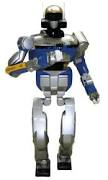
\includegraphics[height=2cm]{hrp2.jpeg}
\hspace{0.5cm}
\includegraphics[height=1cm]{logo/logoAIST.jpeg}\\
}
% - Use the \inst command only if there are several affiliations.
% - Keep it simple, no one is interested in your street address.

\date % (optional, should be abbreviation of conference name)
{JNRH - Toulouse - 2016}
% - Either use conference name or its abbreviation.
% - Not really informative to the audience, more for people (including
%   yourself) who are reading the slides online

\subject{Robotics}
% This is only inserted into the PDF information catalog. Can be left
% out. 


% If you have a file called "university-logo-filename.xxx", where xxx
% is a graphic format that can be processed by latex or pdflatex,
% resp., then you can add a logo as follows:

%\pgfdeclareimage[height=0.5cm]{university-logo}{logo/koroibot-logo}
%\logo{\pgfuseimage{university-logo}}



% Delete this, if you do not want the table of contents to pop up at
% the beginning of each subsection:
%\AtBeginSubsection[]
%{
%  \begin{frame}<beamer>{Outline}
%  \vskip-6ex
%   \tableofcontents[currentsection,currentsubsection]
% \end{frame}
%}

%\AtBeginSection[]
%{
%  \begin{frame}<beamer>{Outline}
%  \vskip-6ex
%      \tableofcontents[currentsection]
%  \end{frame}
%}

\newcommand{\sectionend}{
  \begin{frame}<beamer>{Outline}
    \vskip-6ex
    \tableofcontents[currentsection] 
  \end{frame}
}

\newcommand{\subsectionend}{
  \begin{frame}<beamer>{Outline}
    \vskip-6ex     
    \tableofcontents[currentsection,currentsubsection]
  \end{frame}
}


% If you wish to uncover everything in a step-wise fashion, uncomment
% the following command: 

%\beamerdefaultoverlayspecification{<+->}

\newcommand{\chwithnonumbers}{false}
\newcommand{\bq}{{\bf q}}
\newcommand{\bhq}{{\bf \hat{q}}}
\newcommand{\eq}[1]{(\ref{#1})}
\newcommand{\mbf}[1]{{\mathbf{#1}}}
\newcommand{\deriv}[1]{d#1}

\newcommand{\R}{{\mathbb{R}}}

\newcommand{\md}{d}

% --- Notation --- %
\newcommand{\mProjec}[1]{\mbf{Proj}(#1)}
\newcommand{\mP}[1]{\mbf{P_{#1}}}
\newcommand{\mPaug}[1]{\mbf{P_{#1}^{A}}}
\newcommand{\mProj}[2]{\mbf{P_{#1 \dots #2}}}

\newcommand{\mC}[1]{\mbf{C_{#1}}}

\newcommand{\mL}[1]{\mbf{L_{#1}}}
\newcommand{\mpL}[1]{\mbf{L_{#1}^{+}}}
\newcommand{\maL}[1]{\mbf{\widehat{L}_{#1}}}
\newcommand{\mapL}[1]{\mbf{\widehat{L_{#1}^{+}} }}
\newcommand{\mpaL}[1]{\mbf{\widehat{L}_{#1}^{+}}}
\newcommand{\mLaug}[1]{\mbf{L_{#1}^{A}}}
\newcommand{\mpLaug}[1]{\mbf{L_{#1}^{A+}}}
\newcommand{\mtL}[1]{\mbf{\widetilde{L_{#1}}}}
\newcommand{\mtpL}[1]{\mbf{\widetilde{L_{#1}}^{+}}}

\newcommand{\mJ}[1]{\mbf{J_{#1}}}
\newcommand{\mhJ}[1]{\mbf{\hat{J}_{#1}}}
\newcommand{\mdJ}[1]{\mbf{\dot{J}_{#1}}}
\newcommand{\mpJ}[1]{\mbf{J_{#1}^{+}}}
\newcommand{\maJ}[1]{\mbf{\widehat{J}_{#1}}}
\newcommand{\mapJ}[1]{\mbf{\widehat{J_{#1}^{+}} }}
\newcommand{\mpaJ}[1]{\mbf{\widehat{J}_{#1}^{+}}}
\newcommand{\mJaug}[1]{\mbf{J_{#1}^{A}}}
\newcommand{\mpJaug}[1]{\mbf{J_{#1}^{A+}}}
\newcommand{\mtJ}[1]{\mbf{\widetilde{J_{#1}}}}
\newcommand{\mtpJ}[1]{\mbf{\widetilde{J_{#1}}^{+}}}

\newcommand{\me}[1]{\mbf{e_{#1}}}
\newcommand{\mec}[1]{\mbf{e_{#1}^{*}}}
\newcommand{\medot}[1]{\mbf{\dot{e_{#1}}}}
\newcommand{\meddot}[1]{\mbf{\ddot{e_{#1}}}}
\newcommand{\mde}[1]{\mbf{\md e_{#1}}}

\newcommand{\mte}[1]{\mbf{\widetilde{e}_{#1}}}
\newcommand{\mtedot}[1]{\mbf{\widetilde{\dot{e}_{#1}}}}
\newcommand{\mteddot}[1]{\mbf{\widetilde{\ddot{e}_{#1}}}}

\newcommand{\medotc}[1]{\mbf{\dot{e_{#1}}^{*}}}
\newcommand{\meddotc}[1]{\mbf{\ddot{e_{#1}}^{*}}}

\newcommand{\ms}[1]{\mbf{s_{#1}}}
\newcommand{\msdot}[1]{\mbf{\dot{s_{#1}}}}
\newcommand{\msd}[1]{\mbf{s^{*}_{#1}}}

\newcommand{\mq}{\mbf{q}}
\newcommand{\mqdot}{\mbf{\dot{q}}}
\newcommand{\mqddot}{\mbf{\ddot{q}}}
\newcommand{\mdq}[1]{\mbf{\md q_{#1}}}
\newcommand{\mqr}{\mbf{\rho}}
\newcommand{\mqrlim}{\mbf{\rho}_{lim}}
\newcommand{\mqrdot}{\mbf{\dot{\rho}}}
\newcommand{\mQmax}[1]{\mbf{Q_{#1}}^{MAX}}
\newcommand{\mQmin}[1]{\mbf{Q_{#1}}^{MIN}}

\newcommand{\mr}{\mbf{r}}
\newcommand{\mrdot}{\mbf{\dot{r}}}
\newcommand{\mscrew}{\mbf{v}}

\newcommand{\mres}{\mbf{\rho}}

\newcommand{\mevit}{\mbf{g}^{JointLim}}

\newcommand{\mpot}[1]{V_{#1}}
\newcommand{\mFpot}[1]{\mbf{g}_{#1}}
\newcommand{\mf}[1]{\mbf{f}_{#1}}
\newcommand{\mg}{\mbf{g}}
\newcommand{\mgrad}[1]{{\nabla}_{#1}}
\newcommand{\mgradT}[1]{{\nabla}_{#1}^{\top}}

\newcommand{\qlim}[1]{\bar{q}_{#1}}
\newcommand{\qmin}[1]{\bar{q}^{\min}_{#1}}
\newcommand{\qmax}[1]{\bar{q}^{\max}_{#1}}
\newcommand{\qlmin}[1]{\bar{q}^{\min}_{\ell#1}}
\newcommand{\qlmax}[1]{\bar{q}^{\max}_{\ell#1}}

\newcommand{\mqlim}[1]{\qlim{#1}}
\newcommand{\mqmin}[1]{\qmin{#1}}
\newcommand{\mqmax}[1]{\qmax{#1}}
\newcommand{\mqlmin}[1]{\qlmin{#1}}
\newcommand{\mqlmax}[1]{\qlmax{#1}}


\newcommand{\mvv}{\hbox{\boldmath $v$}}
\newcommand{\mvomega}{\hbox{\boldmath $\omega$}}


\newcommand{\mI}{\mbf{I}}

\newcommand{\derive}[2]{\frac{\deriv{#1}}{\deriv{#2}}}
\newcommand{\dpartial}[2]{\frac{\partial{#1}}{\partial{#2}}}

\newcommand{\mdeuxD}{2-D }
\newcommand{\mtroisD}{3-D }
\newcommand{\mdeuxDd}{2-1/2-D }



\newcommand{\att}[1]{\underline{#1}}

% \newcommand{\argmax}[1]{\arg\!\max_{\!\!\!\!\!\!\!\!\!\!\!\!\!\!\!\!#1}}
\newcommand{\argmax}[1]{\mathop{\arg\!\max}_{#1}}
%\newcommand{\argmax}[1]{\mathop{\mbox{argmax}}_{#1}}
\newcommand{\mdint}{\int\!\!\!\int}


\newcommand{\mCam}{{\bf C}}
\newcommand{\mCamR}{{\bf \psi_c}}

\ifthenelse{\equal{\chwithnonumbers}{true}}{
\newcommand{\newchapter}{\chapter*}
\newcommand{\newsection}{\section*}
\newcommand{\newsubsection}{\subsection*}
}
{
\newcommand{\newchapter}{\chapter}
\newcommand{\newsection}{\section}
\newcommand{\newsubsection}{\subsection}
}

\newcommand{\pcrefc}{PC^{ref}_{c}}
\newcommand{\cpcrefc}{CPC^{ref}_{c}}
\newcommand*\rfrac[2]{{}^{#1}\!/_{#2}}






\newcommand{\I}{\mathbb{I}}

\newcommand{\NT}{\textup{N}}
\newcommand{\NX}{n_\textup{x}}
\newcommand{\NU}{n_\textup{u}}

\newcommand{\FL}{\textup{FL}}
\newcommand{\FR}{\textup{FR}}

\newcommand{\HL}{\textup{HL}}
\newcommand{\HR}{\textup{HR}}

\newcommand{\ini}{\textup{ini}}
\newcommand{\fin}{\textup{fin}}
\newcommand{\tini}{t_{\textup{ini}}}
\newcommand{\tfin}{t_{\textup{fin}}}

\newcommand{\Qf}{{\bf Q}_{i}}
\newcommand{\tauf}{\mathbf{\tau}_i}
\newcommand{\pf}{{\bf p}_{i}}
\newcommand{\ff}{{\bf f}_{i}}
\newcommand{\ffz}{f_{i,z}}
\newcommand{\ffx}{f_{i,x}}
\newcommand{\ffy}{f_{i,y}}
\newcommand{\com}{{\bf c}}
\newcommand{\dcom}{\dot{\bf c}}
\newcommand{\ddcom}{\ddot{\bf c}}
\newcommand{\dddcom}{\dddot{\bf c}}

\newcommand{\ffk}{{\bf f}^k_{i}}
\newcommand{\ffkx}{{\bf f}^k_{i,x}}
\newcommand{\ffky}{{\bf f}^k_{i,y}}
\newcommand{\ffkz}{{\bf f}^k_{i,z}}

\newcommand{\ffkl}{{\bf f}^{k+l}_{i}}
\newcommand{\ffklz}{{\bf f}^{k+l}_{i,z}}


% define matrix and vector commands
\newcommand  {\const}[1]{\mathrm{#1}}
\renewcommand{\vec}  [1]{\mathbf{#1}}
\newcommand  {\mat}  [1]{\mathrm{#1}}

\newcommand*{\Scale}[2][4]{\scalebox{#1}{$#2$}}%
\newcommand*{\Resize}[2]{\resizebox{#1}{!}{$#2$}}%

% Robot model
\newcommand{\robm}{\it model}

% Generalized inertia matrix
\newcommand{\im}{\bf H}

% Centrifugal and Coriolis matrix
\newcommand{\gbf}{\bf C}

% Generalized forces.
\newcommand{\mtau}{\bm \tau}

% Local variables
\newcommand{\mvJi}{{\bf v}_{Ji}}
\newcommand{\mcJi}{{\bf c}_{Ji}}

\newcommand{\BIN}{\begin{bmatrix}}
\newcommand{\BOUT}{\end{bmatrix}}
\newcommand{\am}{\mathcal{L}}
\newcommand{\lm}{\mathcal{K}}

%\includeonly{Section5}
\graphicspath{{./}{../}{../figures/}{../videos/}}


\usepackage{biblatex}
\bibliography{16-jnrh-mnaveau.bib}
\renewcommand{\footnotesize}{\scriptsize}
%
%\tikzset{every picture/.style={font issue=\footnotesize},
%         font issue/.style={execute at begin picture={#1\selectfont}}
%        }

% Show the table of contents at the beginning of every subsection.
\AtBeginSection[]{
    \vspace*{-1cm}
    \frametitle{Table of contents}
    \tableofcontents[current,currentsubsection]
}

 

\begin{document}

\begin{frame}{}
  \titlepage
\end{frame}

% 45 slides :
\section{introduction}
\setcounter{subsection}{1}
\section{Introduction}

\begin{frame}{Skills in manipulation and locomotion\\ are needed}
\begin{center}
  \vspace*{0.7cm}
  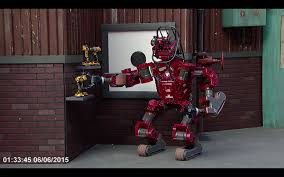
\includegraphics[height=3cm]{darpa/drill.jpeg}
  \hspace*{0.5cm}
  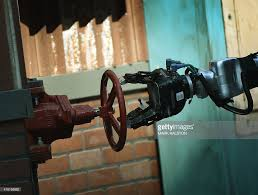
\includegraphics[height=3cm]{darpa/valve.jpeg}\\[0.2cm]
  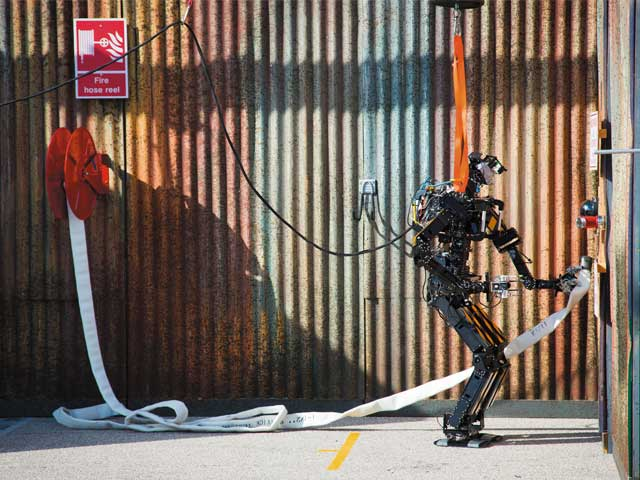
\includegraphics[height=3cm]{darpa/hose.jpg}
\end{center}
%\begin{itemize}
%  \item 
%\end{itemize}
\end{frame}



            % 5

\section{walking}
\setcounter{subsection}{2}
\begin{frame}{Reactive walking pattern generation \only<4>{with obstacles}}
  \vspace*{-1cm}
  \begin{center}
  \scalebox{0.8}{
	\newcommand{\tetazero}{20.55}
	\newcommand{\Fkxzero}{-20}
	\newcommand{\Fkyzero}{20}
	
	\newcommand{\tetaone}{-20}
	\newcommand{\Fkxone}{5}
	\newcommand{\Fkyone}{0}
	
	\newcommand{\tetatwo}{20}
	\newcommand{\Fkxtwo}{25}
	\newcommand{\Fkytwo}{20}
	
	
	\definecolor{color1}{RGB}{1, 121, 111}% corail
	\definecolor{color2}{RGB}{27, 79, 8}% orange 
	\definecolor{color3}{RGB}{237 , 127 ,16}%
	\definecolor{color4}{rgb}{0.9,0.,0.}
	
	\begin{tikzpicture}
		\begin{axis}[xlabel=x,ylabel=y,xmin=-0.2,xmax=0.6,ymin=-0.25,ymax=0.35]
			\only<1>{
			 \addplot[black,thick=2pt,fill=gray!20]
          table{../figures/images/tikz/footstartright.dat};
			}
			\only<1-2>{
        \addplot[black,thick=2pt,fill=gray!20]
          table{../figures/images/tikz/footstartleft.dat};       
			}
			\only<2-3>{
        \addplot[black,thick=2pt,fill=gray!20]
          table{../figures/images/tikz/foot2.dat};
      }
      \only<3-4>{
        \addplot[black,thick=2pt,fill=gray!20]
          table{../figures/images/tikz/foot3.dat};
      }
      \only<4-5>{
        \addplot[black,thick=2pt,fill=gray!20]
          table{../figures/images/tikz/foot4.dat};
			}
			\only<5-6>{
        \addplot[black,thick=2pt,fill=gray!20]
          table{../figures/images/tikz/footendleft.dat};
			}
			\only<6>{
        %\addplot[black,thick=2pt,dashed,fill=white,opacity=0.5]
        \addplot[black,thick=2pt,fill=gray!20]
          table{../figures/images/tikz/footendright.dat};
			}
	    \only<9->{
			  \addplot[black,thick=5pt,fill=gray!20]
			    	table{../figures/images/tikz/footconstraint.dat}; 
  			  \addplot[dashed,black,thick=5pt,fill=gray!20]
			    table{../figures/images/tikz/foot.dat};
			  \addplot[black,very thick,fill=gray!20]
			    table{../figures/images/tikz/footmargin.dat};
	    }
	    	\only<7-8>{
	    	  \addplot[dashed,black,thick=2pt,fill=gray!10,opacity=0.5]
          table{../figures/images/tikz/footstartright.dat};
        \addplot[dashed,black,thick=2pt,fill=gray!10,opacity=0.5]
          table{../figures/images/tikz/footstartleft.dat};
        \addplot[dashed,black,thick=2pt,fill=gray!10,opacity=0.5]
          table{../figures/images/tikz/foot2.dat};
        \addplot[dashed,black,thick=2pt,fill=gray!10,opacity=0.5]
          table{../figures/images/tikz/foot3.dat};
        \addplot[dashed,black,thick=2pt,fill=gray!10,opacity=0.5]
          table{../figures/images/tikz/foot4.dat};
        \addplot[dashed,black,thick=2pt,fill=gray!10,opacity=0.5]
          table{../figures/images/tikz/footendleft.dat};
        \addplot[dashed,black,thick=2pt,fill=gray!10,opacity=0.5]
          table{../figures/images/tikz/footendright.dat};
	    	}
	    	\only<8->{
			  % com
			  \addplot[color1,thick=2pt] table[x index= 0,y index=1]
			    	{../figures/images/tikz/table.dat};
			}
	    	\only<7->{
	      % cop
			  \addplot[color2,thick=5pt] table[x index= 2,y index=3]
			    	{../figures/images/tikz/table.dat}; 
			}
		\end{axis}
	\end{tikzpicture}
	}
	\end{center}
\end{frame}


\begin{frame}{Reactive walking pattern generation \only<4>{with obstacles}}
  \only<4>{\blfootnote{\textbf{Naveau} et al., RA-L 2016}}
  \begin{minipage}{0.48\textwidth}
    Optimization problem solved :
    \vspace*{-0.3cm}
    \begin{equation*}
      \begin{aligned}
        \min_{{\bf U}_k} 
        \sum_{i=0}^{j=4} w_i L_i({\bf U}_{k}) & \\
        {\bf X}_{k+1} = {\bf A}{\bf X}_{k} + {\bf B} {\bf U}_k & \\
        \underline{\bf P} < {\bf P}\only<4>{{\color{red}{({\bf U}_k)}}} {\bf U}_k  < \overline{\bf P}& \\
      \end{aligned}
    \end{equation*}
    with ${\bf U}_k=\begin{pmatrix} \dddot{\bf C}^x_k \; {\bf F}^x_k\; \dddot{\bf C}^y_k \;{\bf F}^y_k \;\only<4>{\color{red}{{\bf \Theta}_k^\mathit{f}}}\end{pmatrix}^T$ \\
  \end{minipage}
  %
  \begin{minipage}{0.48\textwidth}
    \only<1-3>{
      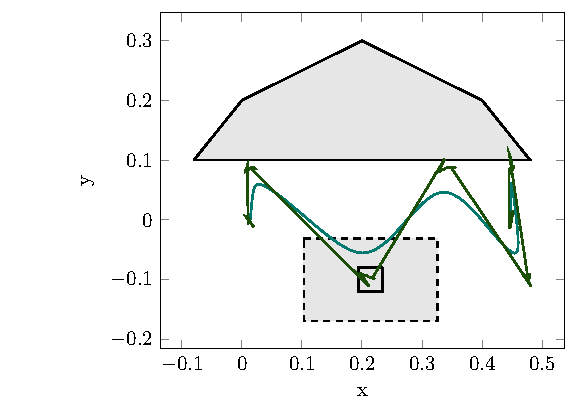
\includegraphics[width=\textwidth]{./images/tikz/convexHulls2}
    }
    \only<4>{
      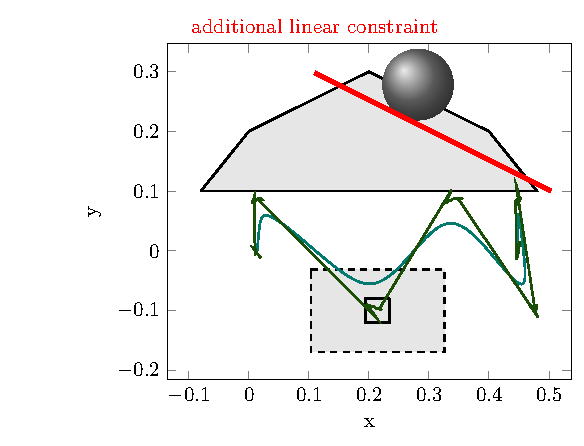
\includegraphics[width=\textwidth]{./images/tikz/convexHullsplusObstacles2}
    }
  \end{minipage}\\
  \vspace*{-0.5cm}
  \begin{center}
  \only<1>{
    {
      \small $L_1({\bf U}_k)$ : linear velocity tracking
%      \begin{equation*}
%        \text{linear velocity tracking : }
%        L_1({\bf U}_k) = \lVert \dot {\bf X}_{k} - {\bf X}_{k}^{ref} \rVert^2_2
%        +  \lVert \dot {\bf Y}_{k} - {\bf Y}_{k}^{ref} \rVert^2_2 
%      \end{equation*}
    }
  }
  \only<2>{
    {
      \small $L_2({\bf U}_k)$ : control norm
%      \begin{equation*}
%        \text{control norm : }
%        L_2({\bf U}_k) = \lVert \dddot {\bf X}_{k} \rVert^2_2
%        + \lVert \dddot {\bf Y}_{k} \rVert^2_2
%      \end{equation*}
    }
  }
  \only<3>{
    {
      \small $L_3({\bf U}_k)$ : balance criteria
%      \begin{equation*}
%        \text{balance criteria : }
%        L_3({\bf U}_k) = \lVert {\bf X}_{k}^{f} - CoP_{k+1}^{x} \rVert^2_2 +
%        \lVert {\bf Y}_{k+1}^{f} - CoP_{k+1}^{y} \rVert^2_2 
%      \end{equation*}
    }
  }
  \only<4>{
    {
      \small $L_4({\bf U}_k)$ : angular velocity tracking
%      \begin{equation*}
%        \text{angular velocity tracking : }
%        L_4({\bf U}_k) = \lVert {\bf \Theta}_{k} 
%        - \int {\bf \Theta}_{k}^{ref} dt \; \rVert_2^2 
%    \end{equation*}
    }
  }
  \end{center}
  
\end{frame}

%%%%%%%%%%%%%%%%%%%%%%%%%%%%%%%%%%%%%%%%%%%%%%%%%%%%%%%%%%%%%%%%%%%%%%%%%%%%%%%


\begin{frame}{SQP Solver}

\begin{itemize}
\item Original nonlinear problem :
  \begin{align*}
    \min_{\color{txtcolor2}{\bf U}_k}  \quad & L({\color{txtcolor2}{\bf U}_k}) \\
    \text{s.t.} \quad & \underline{\bf P} \leq \tilde{\bf P}({\color{txtcolor2}{\bf U}_k}) \leq \overline{\bf P}
  \end{align*}
\item QP approximation :
  \begin{align*}
    \min_{{\color{txtcolor5}{\bf \Delta U}_k}} \quad &
    g({\bf U}_{k-1}) {\color{txtcolor5}{\bf \Delta U}_k} +
    \frac{1}{2} {\color{txtcolor5}{\bf \Delta U}_k}^T H({\bf U}_{k-1}) {\color{txtcolor5}{\bf \Delta U}_k} \\
    \text{s.t.} \quad & \underline{h} - h_{k-1} \leq J({\bf U}_{k-1}) {\color{txtcolor5}{\bf \Delta U}_k} \leq \overline{h} - h_{k-1}\\
    {\color{txtcolor2}{\bf U}_k} =& {\bf U}_{k-1} + \alpha {\color{txtcolor5}{\bf \Delta U}_k}
  \end{align*}
\end{itemize}
\end{frame}

%%%%%%%%%%%%%%%%%%%%%%%%%%%%%%%%%%%%%%%%%%%%%%%%%%%%%%%%%%%%%%%%%%%%%%%%%%%%%%%

\begin{frame}{Dynamic Filter}
\blfootnote{\textbf{Naveau}, Kudruss et al., Humanoids 2014}
\vspace*{-1cm}
  \begin{center}
    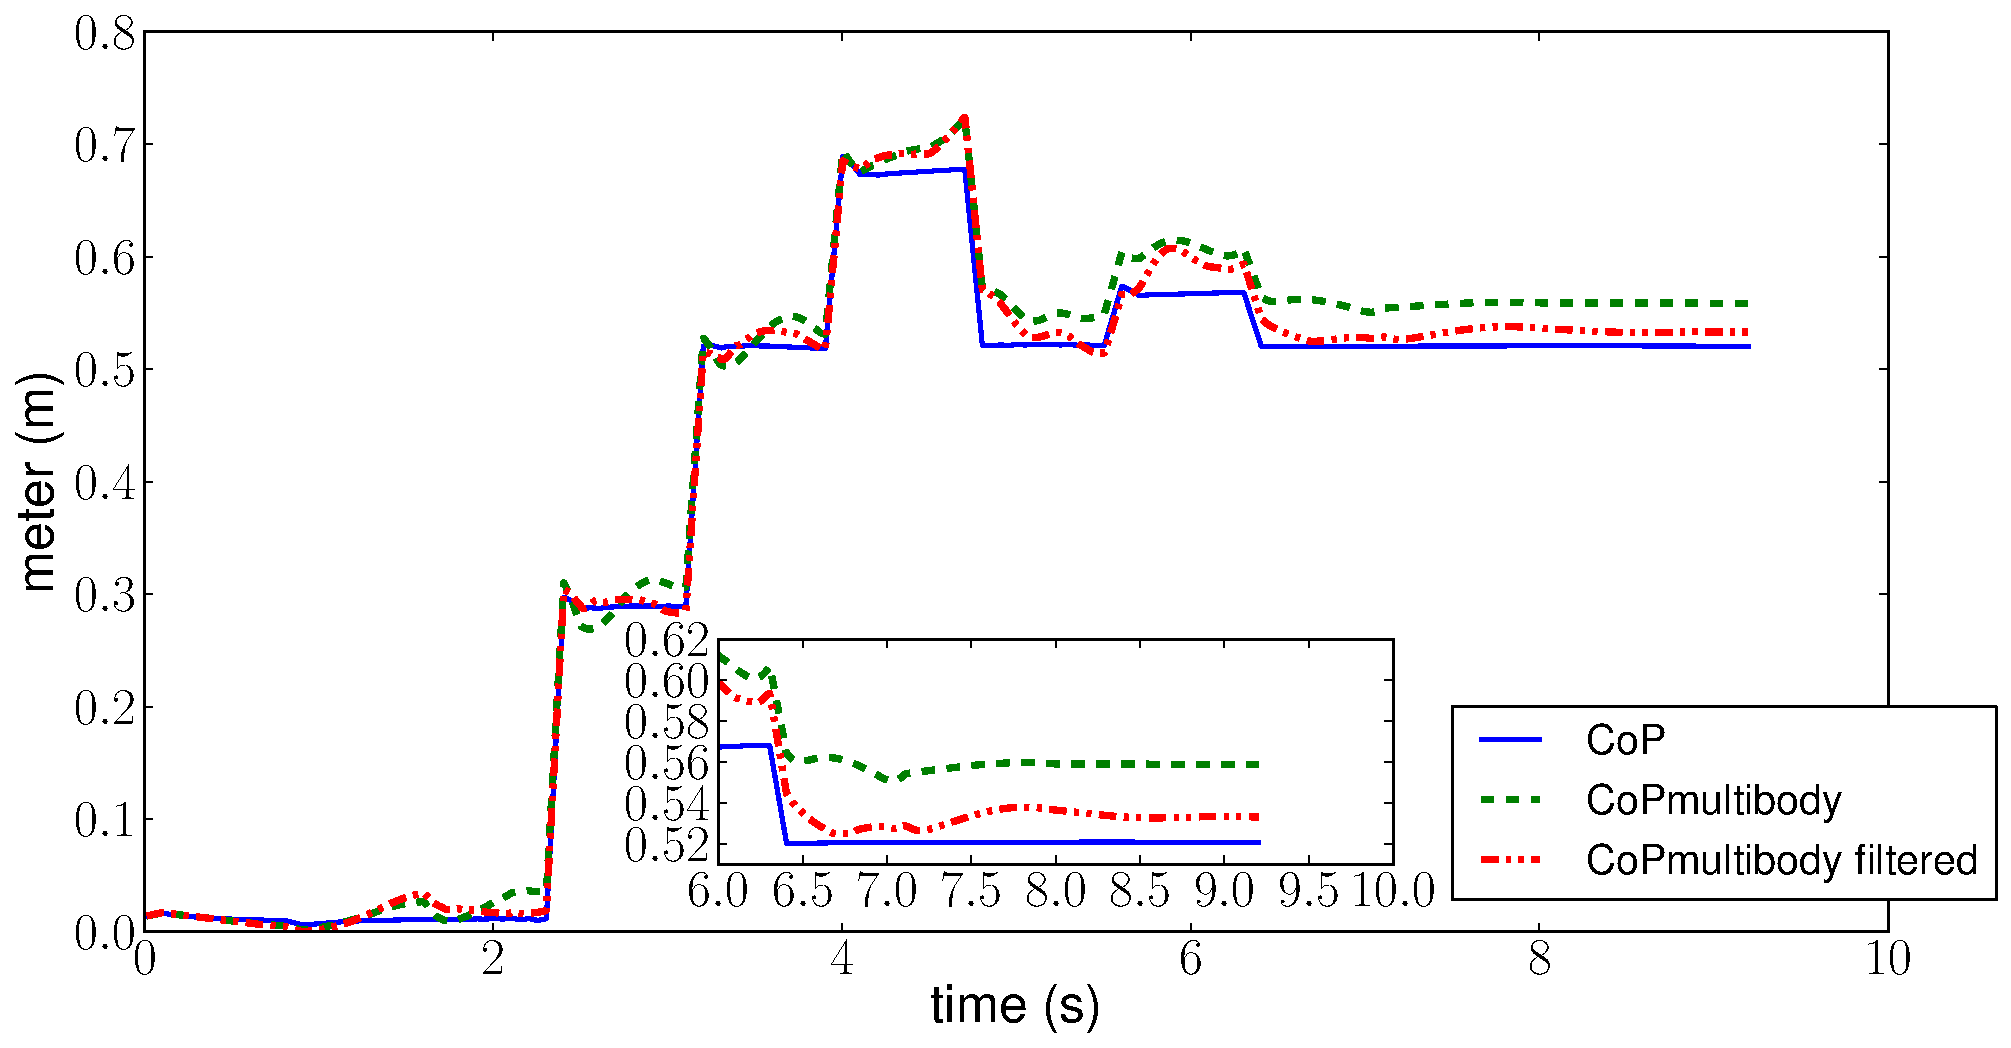
\includegraphics[height=0.8\textheight, keepaspectratio]
      {./figures/nmpc_walkgen/copmbpres.pdf}    
  \end{center}
\end{frame}

%%%%%%%%%%%%%%%%%%%%%%%%%%%%%%%%%%%%%%%%%%%%%%%%%%%%%%%%%%%%%%%%%%%%%%%%%%%%%%%

\begin{frame}{Feedback Scheme}

\begin{center}
  \hspace*{-1cm}
  \scalebox{0.7}{%!TEX root = ../../14-icra-RealTimeNMPC.tex

\tikzstyle{block} = [draw, fill=blue!20, rectangle,
    minimum height=2em, minimum width=5em, align=center]
\tikzstyle{sum} = [draw, fill=blue!20, circle, node distance=1cm]
\tikzstyle{input} = [coordinate]
\tikzstyle{output} = [coordinate]
\tikzstyle{pinstyle} = [pin edge={to-,thin,black}]

% The block diagram code is probably more verbose than necessary
\begin{tikzpicture}[auto, node distance=2cm,>=latex]

    % We start by placing the blocks
    \node [input]  at (0.0, 0.0) (input)  {};
    \node [input]  at (3, 0.0) (velocity) {};
    \node [input]  at (7.2, -2.8) (feedback)  {};
    \node [input]  at (16, -2.8) (feedback2)  {};
    \node []    at ( 0.0, 0.0) (sumin)  {};
    %\node [output]    at ( 15, 0.0) (sumout) {};
    \draw [fill=green,opacity=.2,text opacity=1] (0.1,1.5) rectangle (12.6,-2.0);
    \node at(10,-1.7) {\textcolor{green!20!black!100}{Stack of Tasks}};

%    \node [block] at (4.6,-1.7) (lwc) {
%        Left Wrist\\
%        Hybrid\\
%        Controller        
%    };

%    \node [block] at (1.7,0.0) (walking) {
%        Walking \\
%        Task    
%    };

    \node [block] at (1.7,0) (wpg) {
        Walking\\
        Pattern\\
        Generator
    };
    \node [block, fill=green!30!black!80] at (5.2,0) (dyn) {
        Dynamic\\
        Filter
    };
    \node [block] at (8.5,0) (ttt) {
        Task for\\
        Trajectory\\
        Tracking
    };    
    \node [block] at (11.5,0) (qp) {
        HQP\\
        solver
    };
    \node [block] at (15, 0) (system) {
    		Robot Hardware\\
    		{\footnotesize Simulation/Robot}\\
    		and\\
    		{\footnotesize motion capture system}
    	};

    % PATHS
    	% Forward chaine
%    \draw [draw,-] (input) -- node {\small ${\mathbf{p}}^{\,{\text {ref}}}$} (walking);
    
    \draw [draw,->] ([xshift=-2cm]wpg.west) -- node {\small ${\mathbf v}^{\,{\text{ref}}}$} (wpg);
%    \draw [draw,- ] (walking) -- node {} (velocity);
%    \draw [draw,->] (velocity) |- node {} (lwc);
%    \draw [->] (wpg) -- node {\small $c^{ref},f^{ref}$} (dyn);
%    \draw [->] (dyn) -- node {\small $\tilde{c}^{\,ref},f^{ref}$} (sot);
    \draw [->] (wpg) -- node [text width=1cm]{\small ${\mathbf{p}_{com}}^{\,{\text {ref}}}$ ${\mathbf{p}_{foot}}^{\,{\text {ref}}}$} (dyn);
    
    \draw [->] (dyn) -- node [text width=1cm]{\small ${\tilde{\mathbf{p}}_{com}}^{\,{\text {ref}}}$ ${\mathbf{p}_{foot}}^{\,{\text {ref}}}$} (ttt);
    
    \draw [->] (ttt) -- node [text width=1cm]{
    \small Tasks
    } (qp);
    \draw [->] (qp) -- node [text width=0.6cm]{\small ${\mathbf q}^{\,{\text{ref}}}$ $\dot{{\mathbf q}}^{\,{\text{ref}}}$} (system);
    
%    \draw [->] (lwc) -| node [near start, above]{\small ${\mathbf{p}_{lw}}^{\,{\text {ref}}}$} (ttt);
    %\draw [->] (system) -- node {} (sumout);

    % Feedback chaine
    \draw [- ] ([xshift=+0.8cm]dyn.east) |- node {}
               ([xshift=-0.5cm,yshift=-1.0cm]wpg.west);
    \draw [->] ([xshift=-0.5cm,yshift=-1.0cm]wpg.west) |- node {}
               ([yshift=-0.2cm]wpg.west);
    
%    \draw [- ] (system.east)    -| node {} (feedback2);
%    \draw [- ] (feedback2)  -- node [above]{\small $\mathbf{f}_{lw},\mathbf{p}_{w},\mathbf{p}_{lw},\mathbf{p}_{f}$} (feedback);
%    \draw [->] (3.0,-2.8) |- node [near start, above]{} ([yshift=-0.2cm]lwc.west);
%    \draw [->] (feedback) |- node [below=0.7cm, right]{\small $\mathbf{p}_{ch}$} ([yshift=-0.2cm]walking);

%    \draw [->] (dyn) -| node[above right] {\small $\hat{c}^{\,x,y,\theta}$, $\hat{f}^{\,\,x,y,\theta}$} (wpg);
\end{tikzpicture}
}
\end{center}

\end{frame}

%%%%%%%%%%%%%%%%%%%%%%%%%%%%%%%%%%%%%%%%%%%%%%%%%%%%%%%%%%%%%%%%%%%%%%%%%%%%%%%

\begin{frame}{Experiment on HRP2}
  \begin{center}
    \movie[autostart,loop]{
    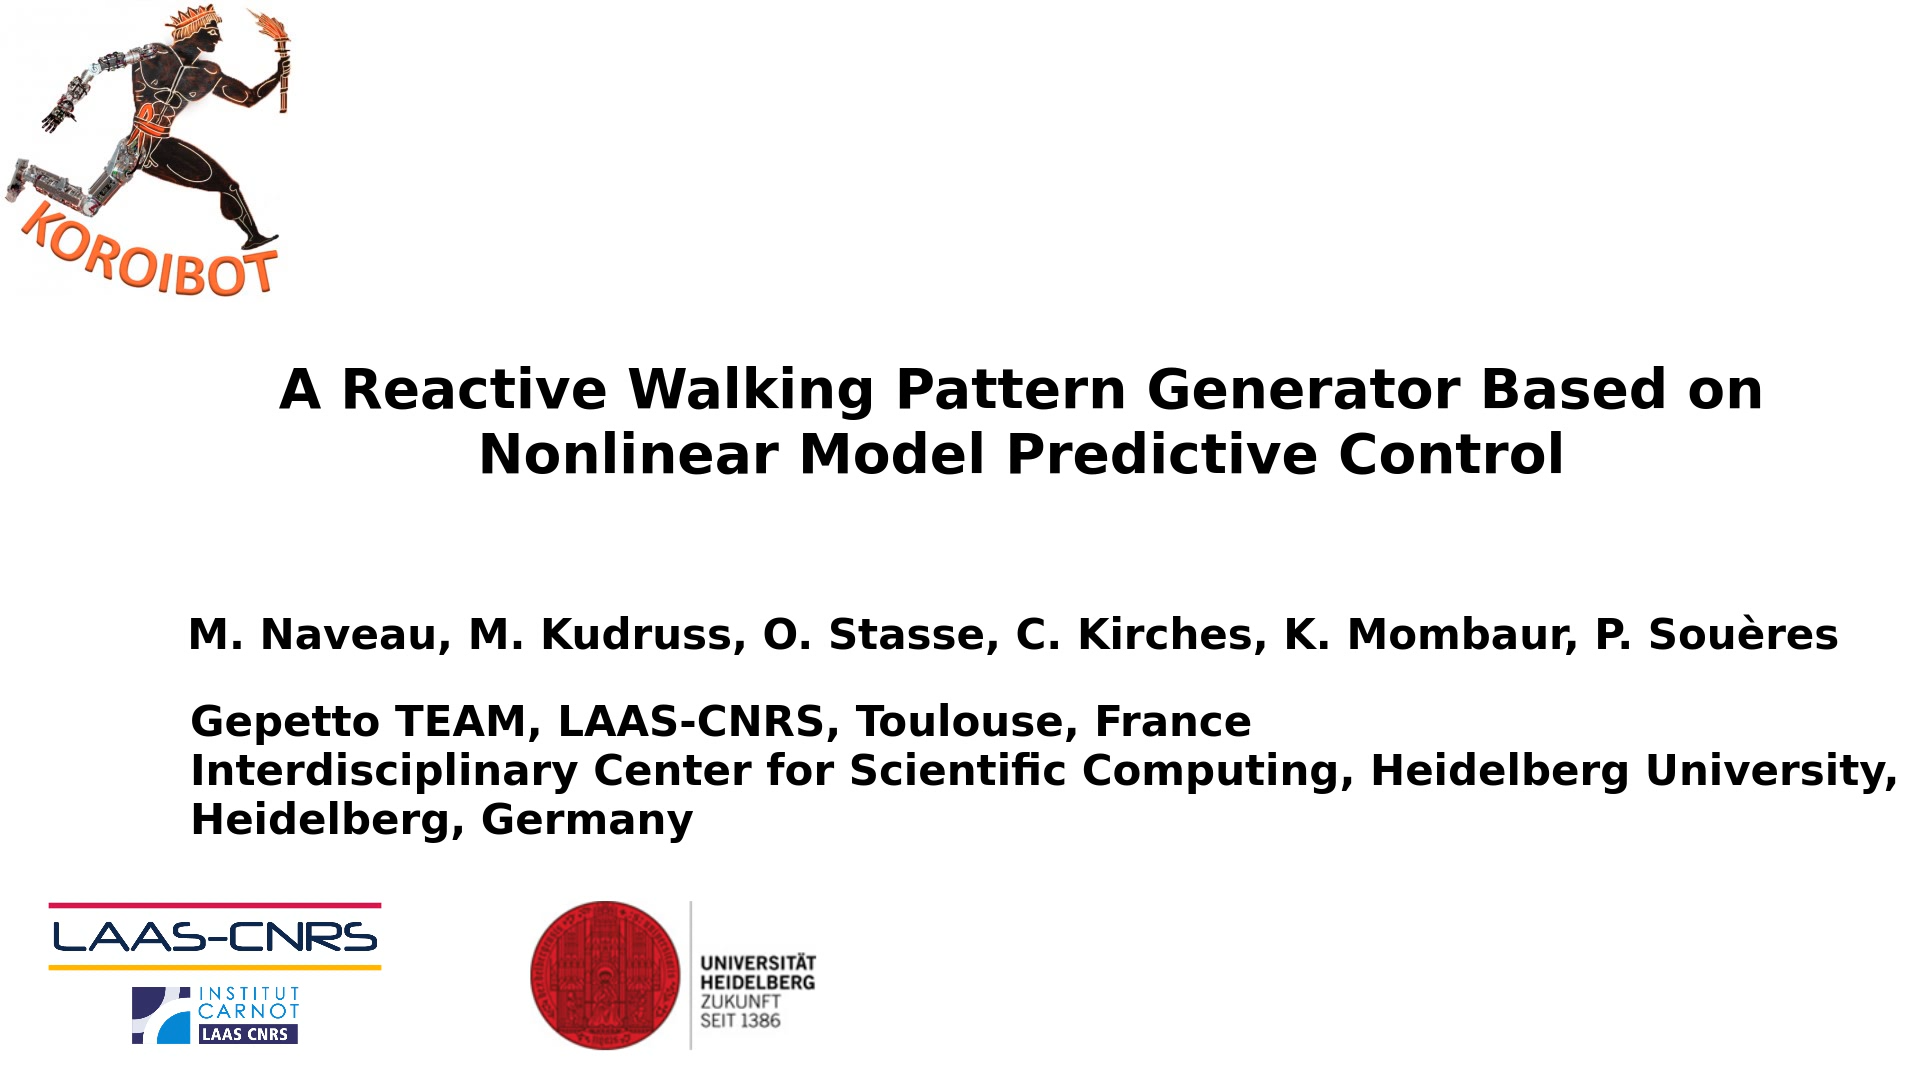
\includegraphics[width=0.85\linewidth, keepaspectratio]
      {16-raletter-NMPC-v19.png}    
    }  
    {videos/16-raletter-NMPC-short.mp4}
  \end{center}
\end{frame}

%%%%%%%%%%%%%%%%%%%%%%%%%%%%%%%%%%%%%%%%%%%%%%%%%%%%%%%%%%%%%%%%%%%%%%%%%%%%%%%

            % 5

\section{multicontact}
\setcounter{subsection}{3}

\begin{frame}{Multicontact Locomotion}
\vspace*{-0.5cm}
\begin{itemize}
 \item Observation : Great energy consumption during climbing stairs
\end{itemize}

\begin{center}
  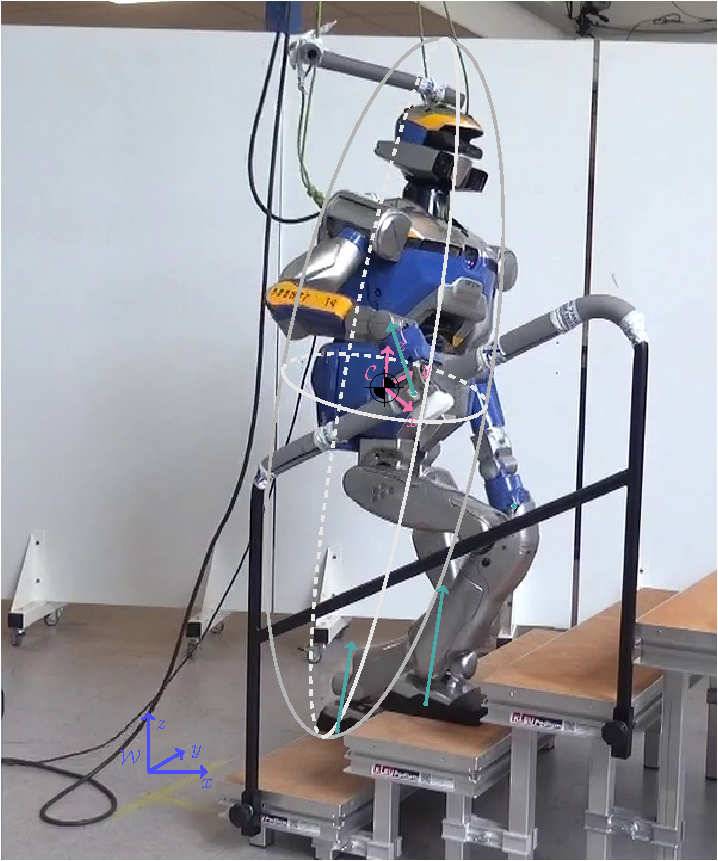
\includegraphics[height=0.6\textheight]{multicontact/cover.pdf}
  \hspace*{0.5cm}
  \begin{minipage}{0.3\linewidth}
    \vspace*{-4.8cm}
    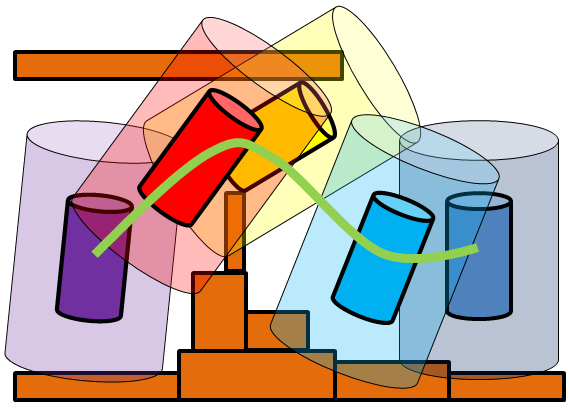
\includegraphics[width=\linewidth]{multicontact/rbprm2.png}\\
    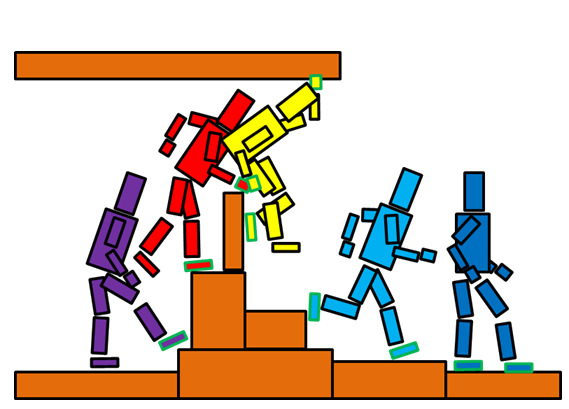
\includegraphics[width=\linewidth]{multicontact/rbprm3.png}  
  \end{minipage}
\end{center}


\begin{itemize}
 \item Hypothesis : Distributing the forces on the whole robot body will decrease the energy consumption
\end{itemize}

\end{frame}

%%%%%%%%%%%%%%%%%%%%%%%%%%%%%%%%%%%%%%%%%%%%%%%%%%%%%%%%%%%%%%%%%%%%%%%%%%%%%%%


\begin{frame}{Centroidal Dynamics}

\begin{itemize}

\item The dynamic constraint \textcolor{txtcolor2}{(M. Kudruss, Humanoids 2015)} :
\begin{scriptsize}
\begin{align*}
  m
  \begin{bmatrix}
  \ddcom - {\bf g} \\
  \com \times (\ddcom - {\bf g})
  \end{bmatrix}
  +
  \begin{bmatrix}
   {\bf 0} \\
     \textcolor{txtcolor2}{{\bf I}_c \dot{\omega}}
  \end{bmatrix}
  =
  \begin{bmatrix}
  \sum_{i=1}^{M}
  \Qf \ff \\
  \sum_{i=1}^{M}
  \pf \times \Qf  \ff
  \end{bmatrix}
\end{align*}
\end{scriptsize}
\item the state :
$
\begin{bmatrix}
\com & \dcom & \textcolor{txtcolor2}{\omega}
\end{bmatrix}^T
$
\item the controls :
$
\begin{bmatrix}
\ff
\end{bmatrix}^T
$

\textcolor{txtcolor1}{\hrule}
\vspace*{0.5cm}

\item The dynamic constraint \textcolor{txtcolor5}{(J. Carpentier, ICRA 2016)} :
\begin{scriptsize}
\begin{align*}
  m
  \begin{bmatrix}
  \ddcom - {\bf g} \\
  \com \times (\ddcom - {\bf g})
  \end{bmatrix}
  +
  \begin{bmatrix}
   {\bf 0} \\
   \textcolor{txtcolor5}{ \dot{\bf \am} }
  \end{bmatrix}
  =
  \begin{bmatrix}
  \sum_{i=1}^{M}
  \Qf \ff \\
  \sum_{i=1}^{M}
  \pf \times \Qf  \ff +
  \textcolor{txtcolor5}{ \Qf \tauf}
  \end{bmatrix}
\end{align*}
\end{scriptsize}
\item the state :
$
\begin{bmatrix}
\com & {\bf h}=m\dcom & \textcolor{txtcolor5}{\mathcal{L}}
\end{bmatrix}^T
$
\item the controls :
$
\begin{bmatrix}
\ff & \textcolor{txtcolor5}{\tauf}
\end{bmatrix}^T
$

\end{itemize}

\end{frame}

%%%%%%%%%%%%%%%%%%%%%%%%%%%%%%%%%%%%%%%%%%%%%%%%%%%%%%%%%%%%%%%%%%%%%%%%%%%%%%%

\begin{frame}{The optimal control problem}
\vspace*{-0.5cm}
\begin{columns}
\begin{column}{0.5\textwidth}

\begin{itemize}
  \item {(M. Kudruss, Humanoids 2015)}
\end{itemize}

\begin{itemize}
  \item Cost Functions :
  \begin{itemize}
    \item Linear/Angular velocity
    \item \textcolor{blue!70!black}{CoM attracted by all contacts}
    \item Controls (forces)
    \item \textcolor{blue!70!black}{Fixed sequence timing}
    \item Linear/Angular acceleration
  \end{itemize}
  \vspace*{0.5cm}
  \item Constraints :
  \begin{itemize}
    \item \textcolor{blue!70!black}{Kinematic Constraints}
    \item \textcolor{blue!70!black}{3D Friction Cone}
  \end{itemize}
\end{itemize}
%
%\begin{subequations}
%\begin{eqnarray*}
%\hspace{0em}	\underset{\substack{\hspace{0.2em} \underline{\bm x}, \; \underline{\bm u}} }{\min } \ \ \
%	& & \hspace{-4em} \int_{0}^{T}
%%	{\scriptstyle
%	  \textcolor{red!70!black}{||\dcom||^2_2 +
%	  ||{\omega}||^2_2} +
%    \textcolor{orange!70!black}{\ell_2\,_{kin}} \\
%    & & \hspace{-3em} +
%    \textcolor{green!50!black}{||{\dot{\omega}}||^2_2} +
%    \textcolor{purple!100!blue!100}{||{\ddcom}||^2_2}
%%  }
%  dt  \\[1em]
%	s.t.
%	&  \forall t,i& \ff \in \mathcal{K}_i^{\textcolor{blue!50!green!100!black}{3D}} \\
%  &  \forall t& \textcolor{orange!70!black}{\com ,\; \dcom} ,\; {\omega} \in \mathcal{B}_x \\ 
%  &  \forall t,i& {\ff ,\; {\sigma}} \in \mathcal{B}_u    \\[1em]
%  & \forall t & \dot{\bm{x}} = {dyn}(\bm x, \bm u)  \\	
%	& & \hspace{-4em} \bm x(0) = \bm x_{0} \; ; \; \bm x(T) \in \mathcal{X}_* 
%\end{eqnarray*}
%\end{subequations}

\end{column}
%
{\color{txtcolor2}\vrule}
%
%
\begin{column}{0.5\textwidth}

\begin{itemize}
\item {(J. Carpentier, ICRA 2016)}
\end{itemize}

\begin{itemize}
  \item Cost Functions :
  \begin{itemize}
    \item {Linear Momentum}
    \item \textcolor{blue!70!black}{CoM rejected by all contacts}
    \item {Controls (forces and torques)}
    \item \textcolor{blue!70!black}{Free sequence timing}
    \item {Linear/Angular momentum derivatives}
  \end{itemize}
  \item Constraints :
  \begin{itemize}
    \item \textcolor{blue!70!black}{No Kinematics Hard Constraints}
    \item \textcolor{blue!70!black}{6D Friction Cone}
  \end{itemize}
\end{itemize}

%
%\begin{subequations}
%\begin{eqnarray*}
%\hspace{0em}	\underset{\substack{\hspace{0.2em} \underline{\bm x}, \; \underline{\bm u}} }{\min } \ \ \  
%	& & \hspace{-4em} \int_{0}^{T}
%%	{\scriptstyle
%    \textcolor{red!70!black}{||m\dcom||^2_2} +
%  	  \textcolor{orange!70!black}{\text{exp}_{kin}} \\
%  	  & & \hspace{-3em} +
%    \textcolor{green!50!black}{||{\dot{\mathcal{L}}}||^2_2} +
%	  \textcolor{purple!100!blue!100}{||{\ff}||^2_2} +
% 	  \textcolor{purple!100!blue!100}{||{\tauf}||^2_2} 
%%  }
%  dt  \\[1em]
%	s.t.
%	&  \forall t,i& [\ff \;\; {\tauf}] \in \mathcal{K}_i^{\textcolor{blue!50!green!100!black}{6D}} \\
%  &  \forall t& {{\mathcal{L}}} \in \mathcal{B}_{\mathcal{L}}    \\ 
%  &  \forall t& {\ff ,\; {\tauf}} \in \mathcal{B}_u    \\ [1em]
%  & \forall t,i & \dot{\bm{x}} = {dyn}(\bm x, \bm u)  \\	
%	& & \hspace{-4em} \bm x(0) = \bm x_{0} \; ; \; \bm x(T) \in \mathcal{X}_* 
%\end{eqnarray*}
%\end{subequations}

\end{column}
\end{columns}


\end{frame}

%%%%%%%%%%%%%%%%%%%%%%%%%%%%%%%%%%%%%%%%%%%%%%%%%%%%%%%%%%%%%%%%%%%%%%%%%%%%%%%

\begin{frame}{Experiment on HRP2}
  \begin{center}
    \movie[autostart,loop]{
    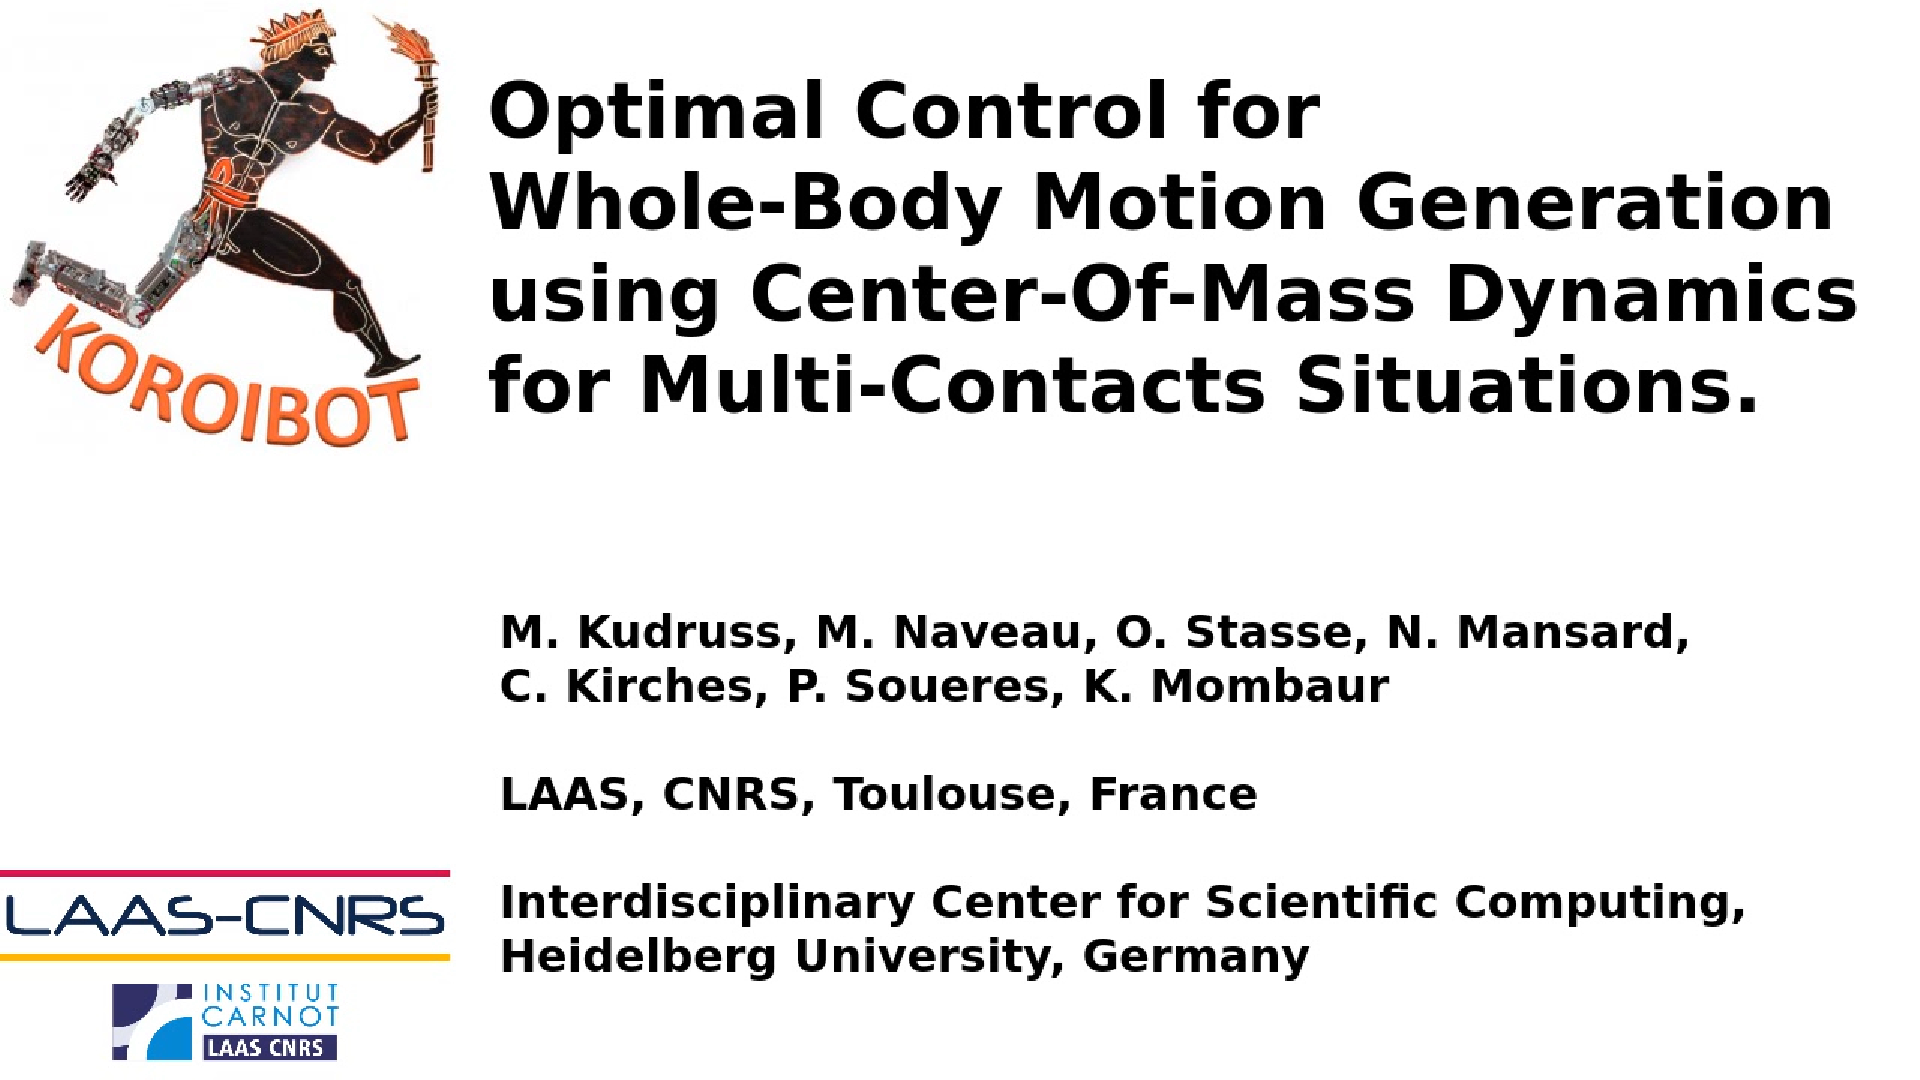
\includegraphics[width=0.8\linewidth, keepaspectratio]
      {multicontact/15-ichr-multicontact.png}
    }  
    {videos/multicontact-short.mp4}
  \end{center}
  \vspace*{-0.5cm}
  \blfootnote{Kudruss, \textbf{Naveau} et al. Humanoids 2015)}
  \blfootnote{Carpentier, Tonneau, \textbf{Naveau} et al. ICRA 2016)}
\end{frame}

%%%%%%%%%%%%%%%%%%%%%%%%%%%%%%%%%%%%%%%%%%%%%%%%%%%%%%%%%%%%%%%%%%%%%%%%%%%%%%%



%\begin{equation}
%  m
%  \begin{bmatrix}
%  \ddcom - {\bf g} \\
%  \com \times (\ddcom - {\bf g})
%  \end{bmatrix}
%  +
%  \begin{bmatrix}
%  {\bf 0} \\
%  \tikz[baseline]{
%      \node[anchor=base] (l) {$ \dot{\mathcal{L}} $} ;
%      %
%      \draw [draw,-,color=red!50,thick] ([xshift=-0.2cm,yshift= 0.2cm]l.center) -- node {}     ([xshift= 0.2cm,yshift=-0.2cm]l.center);
%      %
%      \draw [draw,-,color=red!50,thick] ([xshift=-0.2cm,yshift=-0.2cm]l.center) -- node {}     ([xshift= 0.2cm,yshift= 0.2cm]l.center);
%    }
%  \end{bmatrix}
%  =
%  \begin{bmatrix}
%  \sum_{i=1}^{M}
%  \Qf \ff \\
%  \sum_{i=1}^{M}
%  \pf \times \Qf  \ff
%  \end{bmatrix}
%\end{equation}            % 5

\section{pulling-a-hose}
\setcounter{subsection}{4}
%%%%%%%%%%%%%%%%%%%%%%%%%%%%%%%%%%%%%%%%%%%%%%%%%%%%%%%%%%%%%%%%%%%%%%%%%%%%%%%
%     Problem setup
%%%%%%%%%%%%%%%%%%%%%%%%%%%%%%%%%%%%%%%%%%%%%%%%%%%%%%%%%%%%%%%%%%%%%%%%%%%%%%%

%\begin{frame}{Pulling hose problem}
%%
%  \begin{minipage}{0.55\textwidth}
%    \begin{center}
%      \movie[autostart,loop,continue]{
%        \includegraphics[width=\linewidth, height=\textheight, keepaspectratio]
%        {hose_xp/withoutwalkingtask.png}
%      }
%      {./videos/wihtoutwalkingtask.mpg}
%    \end{center}
%  \end{minipage}  \hfill
%%
%\only<1>{
%  \begin{minipage}{0.42\textwidth}
%    \textbf{\color{txtcolor2} Setup :}
%    \begin{itemize}
%      \item HRP-2 humanoid robot
%      \item rigid, \emph{empty} fire hoze
%      \item motion capture system
%    \end{itemize}
%  \end{minipage}
%}
%%
%\only<2>{
%  \begin{minipage}{0.41\textwidth}
%    \textbf{\color{txtcolor2} Major technical issues while}
%    \begin{itemize}
%%
%    \item \textbf{\color{txtcolor2} pulling :}
%    \begin{itemize}
%      \item Important drift
%      \item Robot less balanced
%    \end{itemize}
%%    
%    \item \textbf{\color{txtcolor2} picking :}
%      \begin{itemize}
%        \item Self-collision
%        \item Joint limit
%        \item Balance
%      \end{itemize}
%%    
%    \end{itemize}
%  \end{minipage}
%}
%%
%\only<3>{
%  \begin{minipage}{0.39\textwidth}
%    \textbf{\color{txtcolor2} Objectives :}
%    \begin{itemize}
%      \item Pick up a rigid fire hose
%      \item Pull it toward a desired position
%    \end{itemize}
%    \vspace*{0.7cm}
%  \end{minipage}
%}
%
%\end{frame}
 
\begin{frame}{Pulling hose problem}
\framesubtitle{(AIST, LAAS-CNRS)}
%
  \begin{center}
    \movie[autostart,loop,continue]{
      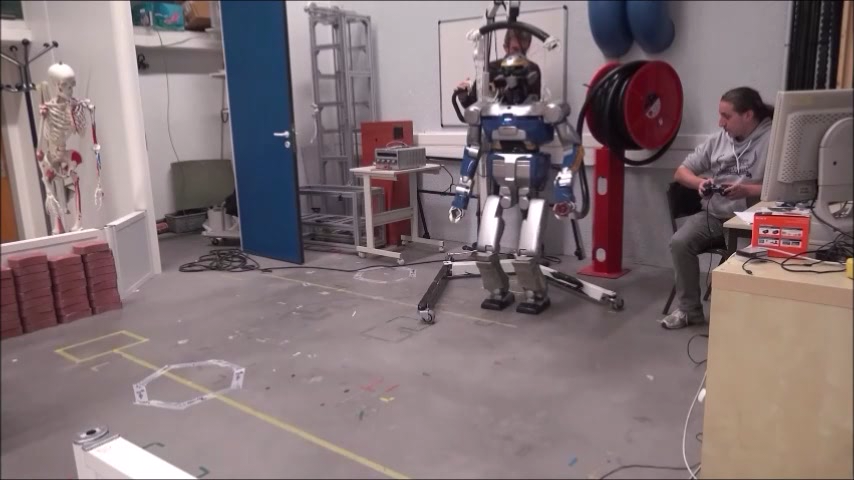
\includegraphics[height=0.5\textheight, keepaspectratio]
      {hose_xp/withoutwalkingtask.png}
    }
    {./videos/wihtoutwalkingtask.mpg}\\
  \end{center}
  \textbf{\color{txtcolor2} Major technical issues :}\\
  \begin{minipage}{0.48\textwidth}
    \begin{itemize}
      \item \textbf{\color{txtcolor2} pulling :}
      \begin{itemize}
        \item Important drift
        \item Robot less balanced
      \end{itemize}
    \end{itemize}
  \end{minipage}
%    
  \begin{minipage}{0.48\textwidth}
    \begin{itemize}
      \item \textbf{\color{txtcolor2} picking :}
      \begin{itemize}
        \item Self-collision
        \item Joint limit
        \item Balance
      \end{itemize}
    \end{itemize}
  \end{minipage}
%

\end{frame} 
 
%%%%%%%%%%%%%%%%%%%%%%%%%%%%%%%%%%%%%%%%%%%%%%%%%%%%%%%%%%%%%%%%%%%%%%%%%%%%%%%%%%%%%%%%
%
%\begin{frame}{Pick Up Motion}
%  \vspace*{0.6cm}
%  \begin{center}
%    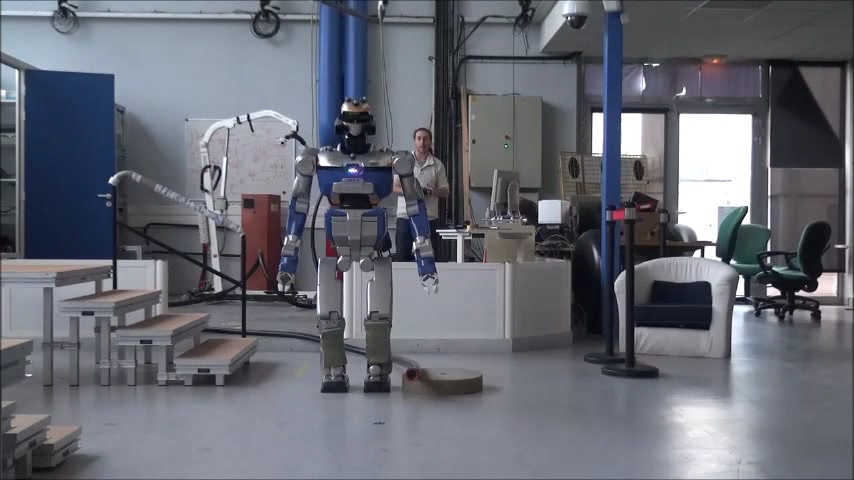
\includegraphics[height = 4.0cm]{hose_xp/pickup.png}
%  \end{center}
%%
%  \vspace*{-1ex}
%  \textbf{\color{txtcolor2} Planning constraint using HPP :}\\
%%  
%  \begin{minipage}{0.45\textwidth}
%    \begin{itemize}
%      \item Static Balance
%      \item Feet flat on the floor
%      \item Left wrist position
%    \end{itemize}
%  \end{minipage}
%%
%  \begin{minipage}{0.50\textwidth}
%    \begin{itemize}
%      \item Robot facing forward
%      \item Close from half-sitting position
%    \end{itemize}
%    \vspace*{0.4cm}    
%  \end{minipage}
%%
%  \begin{center}
%    \small{\color{txtcolor3}\url{https://humanoid-path-planner.github.io/hpp-doc}}
%  \end{center}
%%
%\end{frame}
%
%%%%%%%%%%%%%%%%%%%%%%%%%%%%%%%%%%%%%%%%%%%%%%%%%%%%%%%%%%%%%%%%%%%%%%%%%%%%%%%%%%%%%%%%
%
%\begin{frame}{Walking task}
%  \vspace*{0.2cm}
%  \begin{center}
%    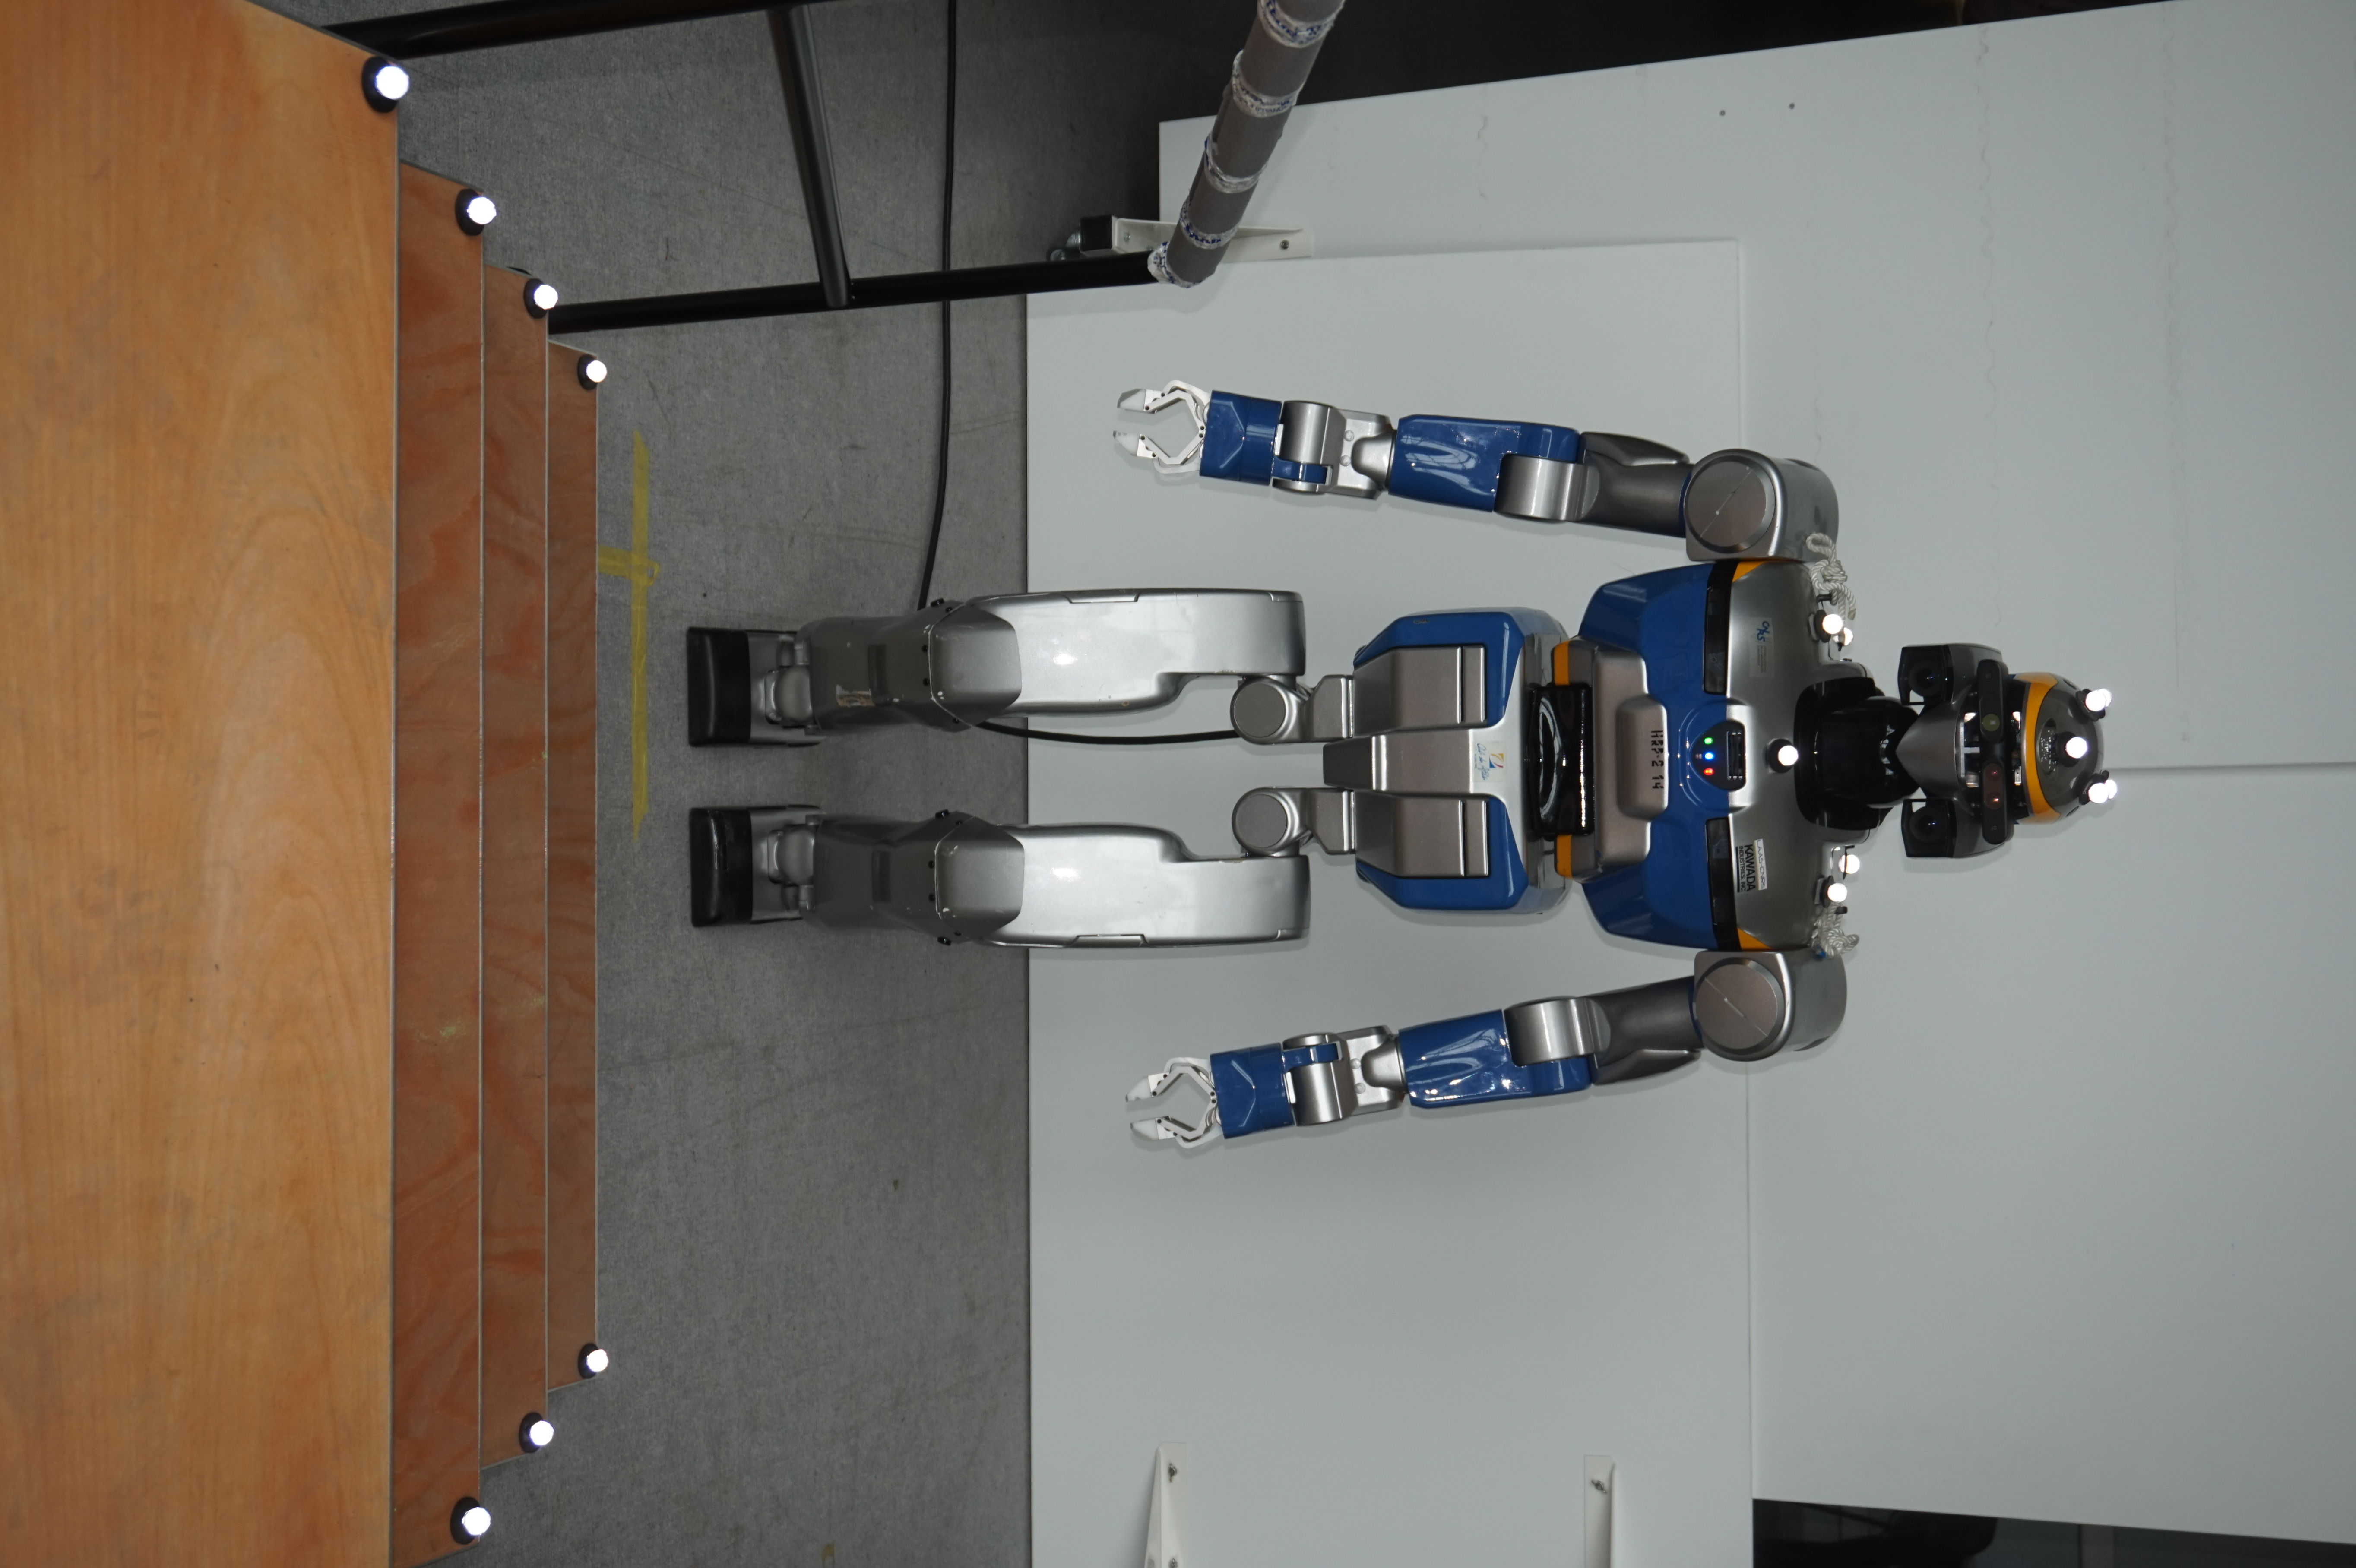
\includegraphics[angle=90, height=0.25\paperheight]{./DSC00610.JPG}
%    \hspace*{1.5cm}
%    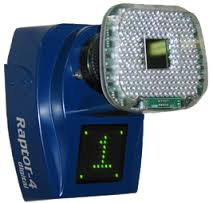
\includegraphics[height=0.25\paperheight]{./camera_raptor.jpeg}
%  \end{center}
%
%  \tikzstyle{na} = [baseline=-.5ex]
%  \begin{itemize}
%    \item adaptive gains
%      \tikz[na] \node[coordinate] (l) {};
%    \item referenced velocity 
%      \tikz[na] \node[coordinate] (vr) {};
%  \end{itemize}
%%
%%  \vspace*{-0.5cm}
%  \begin{align*}
%    \;\;\;\;\;\;\;\;\;\;\;\;\;\;\;\;\;\;\;\;\;\;\;\;\;
%    \tikz[baseline]{
%      \node[fill=txtcolor1,anchor=base] (v)
%      { $ \mathbf{v}^{\mathrm{ref}} $ };
%    }
%    = - \tikz[baseline]{
%      \node[fill=txtcolor2,anchor=base] (l1)
%      {$\lambda$};
%    } \;
%    \tikz[baseline]{
%      \node[fill=txtcolor3,anchor=base] (e1)
%      {$ \mathbf{e}_{w} $};
%    } - 
%    \tikz[baseline]{
%      \node[fill=txtcolor2,anchor=base] (l2)
%      {$ \mathbf{\Lambda} $};
%    }
%    \int \tikz[baseline]{
%      \node[fill=txtcolor3,anchor=base] (e2)
%      {$ \mathbf{e}_{w} $};
%    } dt
%  \end{align*}
%
%  \begin{itemize}
%    \item $ 
%     \tikz[baseline]{
%      \node[fill=txtcolor3,anchor=base] (e3)
%      {$ \mathbf{e}_{w} $};
%    }
%     = 
%     \begin{bmatrix}
%       x_{chest} & y_{chest} & \theta_{chest}
%     \end{bmatrix}^T
%     -$\tikz[na] \node[coordinate] (e) {};\\
%     $
%     \begin{bmatrix}
%       x^{des}_{chest} & y^{des}_{chest} & \theta^{des}_{chest}
%     \end{bmatrix}^T $
%  \end{itemize}
%%
%% Now it's time to draw some edges between the global nodes. Note that we
%% have to apply the 'overlay' style.
%  \begin{tikzpicture}[overlay]
%    \path[->,line width=0.5mm, txtcolor1] (vr) edge [bend left] (v);
%    \path[->,line width=0.5mm, txtcolor3] (e) edge [bend right] (e1);
%    \path[->,line width=0.5mm, txtcolor3] (e) edge [bend right] (e2);
%    \path[->,line width=0.5mm, txtcolor2] (l) edge [bend left] (l1);
%    \path[->,line width=0.5mm, txtcolor2] (l) edge [bend left] (l2);
%  \end{tikzpicture}
%%  
%\end{frame}
%
%
%%%%%%%%%%%%%%%%%%%%%%%%%%%%%%%%%%%%%%%%%%%%%%%%%%%%%%%%%%%%%%%%%%%%%%%%%%%%%%%%%%%%%%%%
%
%\begin{frame}{Hybrid controller}
%  \tikzstyle{na} = [baseline=-0.5ex]
%  \begin{center}
%    \includegraphics[width=0.45\textwidth]
%    {hose_xp/force_Z_feet_withoutController_zoomEnd.pdf}\hfill
%    \includegraphics[width=0.45\textwidth]
%    {hose_xp/force_Z_feet_withController_zoomEnd.pdf}\\
%    \textbf{\color{txtcolor1} without the controller}
%    \tikz[na] \node[coordinate] (without) {};
%    \hfill
%    \tikz[na] \node[coordinate] (with) {};    
%    \textbf{\color{txtcolor1} with the controller}
%    \hfill \hfill
%  \end{center}  
%  
%  \begin{tikzpicture}[overlay]
%    \path[->,line width=0.5mm, txtcolor1] (without) edge (with);
%  \end{tikzpicture}
%  \vspace*{-1cm}
%
%%  \tikzstyle{na} = [baseline=-0.5ex]
%%   \tikz[na] \node[coordinate] (nfpull) {};
%%  desired force \tikz[na] \node[coordinate] (nfd) {};
%%  external force \tikz[na] \node[coordinate] (nflw) {};
%%  left wrist velocity and acceleration \tikz[na] \node[coordinate] (nav) {};
%
%%  
%%  \begin{itemize}
%%    \item pulling force
%%      \tikz[na] \node[coordinate] (nfpull) {};
%%    \item desired force
%%      \tikz[na] \node[coordinate] (nfd) {};
%%    \item wrist measured \\external force 
%%      \tikz[na] \node[coordinate] (nflw) {};
%%  \end{itemize}
%%
%\begin{small}
%  \begin{align*}
%    m & \tikz[baseline]{
%      \node[fill=txtcolor1,anchor=base] (a)
%      { $ \ddot{\bf lw}^{x} $ };
%    }
%   + c \tikz[baseline]{
%      \node[fill=txtcolor1,anchor=base] (v)
%      {$ \dot{\bf lw}^{x} $};
%    } = 
%    \tikz[baseline]{
%      \node[fill=txtcolor4,anchor=base] (flw)
%      {$ {\bf f}_{lw}^{x} $};
%    } + 
%    \tikz[baseline]{
%      \node[fill=txtcolor2,anchor=base] (fd)
%      {$ {\bf f}_{d}^{x} $};
%    } + 
%    \tikz[baseline]{
%      \node[fill=txtcolor3,anchor=base] (fpull)
%      {$ {\bf f}_{pull}^{x} $};
%    }
%    %
%    \\
%    %
%    m & \tikz[baseline]{
%      \node[fill=txtcolor1,anchor=base] (a)
%      { $ \ddot{\bf lw}^{z} $ };
%    }
%   + c \tikz[baseline]{
%      \node[fill=txtcolor1,anchor=base] (v)
%      {$ \dot{\bf lw}^{z} $};
%    } = 
%    \tikz[baseline]{
%      \node[fill=txtcolor4,anchor=base] (flw)
%      {$ {\bf f}_{lw}^{z} $};
%    } + 
%    \tikz[baseline]{
%      \node[fill=txtcolor2,anchor=base] (fd)
%      {$ {\bf f}_{d}^{z} $};
%    } + 
%    \tikz[baseline]{
%      \node[fill=txtcolor3,anchor=base] (fpull)
%      {$ {\bf f}_{pull}^{z} $};
%    }
%    %
%    \\
%    %
%    &\tikz[baseline]{
%      \node[fill=txtcolor1,anchor=base] (a)
%      { $ {\bf lw}^{y} $ };
%    } = {\bf waist}^{y} + \text{offset}
%  \end{align*}
%\end{small}
%%  \begin{itemize}
%%    \item left wrist velocity\\
%%    and acceleration \tikz[na] \node[coordinate] (nav) {};
%%  \end{itemize}
%
%% Now it's time to draw some edges between the global nodes. Note that we
%% have to apply the 'overlay' style.
%%  \begin{tikzpicture}[overlay]
%%    \path[->,line width=0.5mm, txtcolor1]  (nav) edge [bend right] (a);
%%    \path[->,line width=0.5mm, txtcolor1]  (nav) edge [bend right] (v);
%%    \path[->,line width=0.5mm, txtcolor4]   (nflw) edge [bend left] (flw);
%%    \path[->,line width=0.5mm, txtcolor2](nfd) edge [bend left] (fd);
%%    \path[->,line width=0.5mm, txtcolor3]   (nfpull) edge [bend left] (fpull);
%%  \end{tikzpicture}
%  
%\end{frame}


%%%%%%%%%%%%%%%%%%%%%%%%%%%%%%%%%%%%%%%%%%%%%%%%%%%%%%%%%%%%%%%%%%%%%%%%%%%%%%%%%%%%%%%

\begin{frame}{3 combined controllers}
%
  \begin{minipage}{0.30\textwidth}
    \begin{center}
      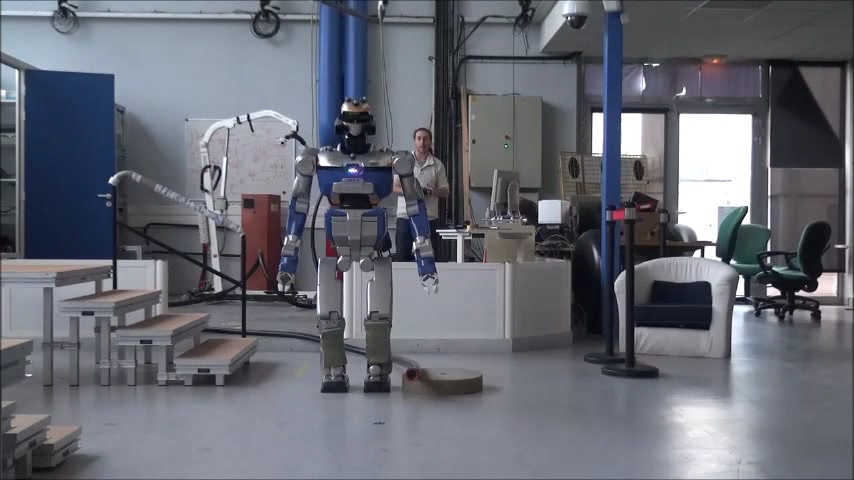
\includegraphics[trim={7.0cm 2.0cm 10.5cm 2.0cm}, clip, height=0.30\textheight]
      {hose_xp/pickup.png}
      %trim={<left> <lower> <right> <upper>}
    \end{center}
  \end{minipage}
%
{\color{txtcolor2}\vrule}
  \begin{minipage}{0.30\textwidth}
    \begin{center}
      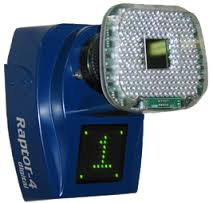
\includegraphics[height=0.20\textheight]{./camera_raptor.jpeg}
    \end{center}
  \end{minipage}
%
{\color{txtcolor2}\vrule}    
  \begin{minipage}{0.35\textwidth}
    \begin{center}
      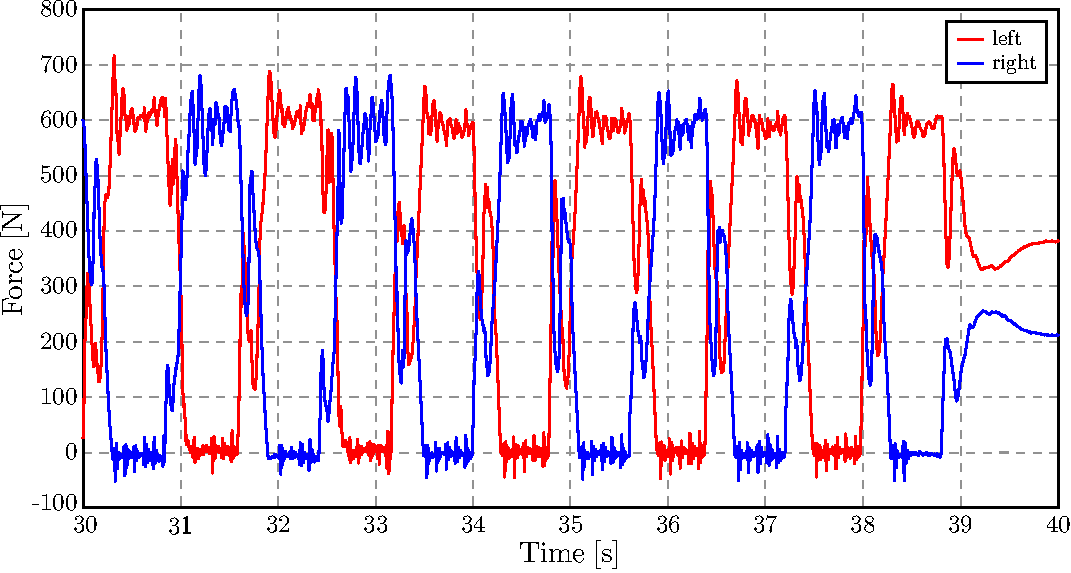
\includegraphics[trim={5.0cm 1.5cm 7.0cm 1.0cm}, clip, width=\textwidth , height=0.15\textheight]
      {hose_xp/force_Z_feet_withoutController_zoomEnd.pdf}\\[1.ex]
      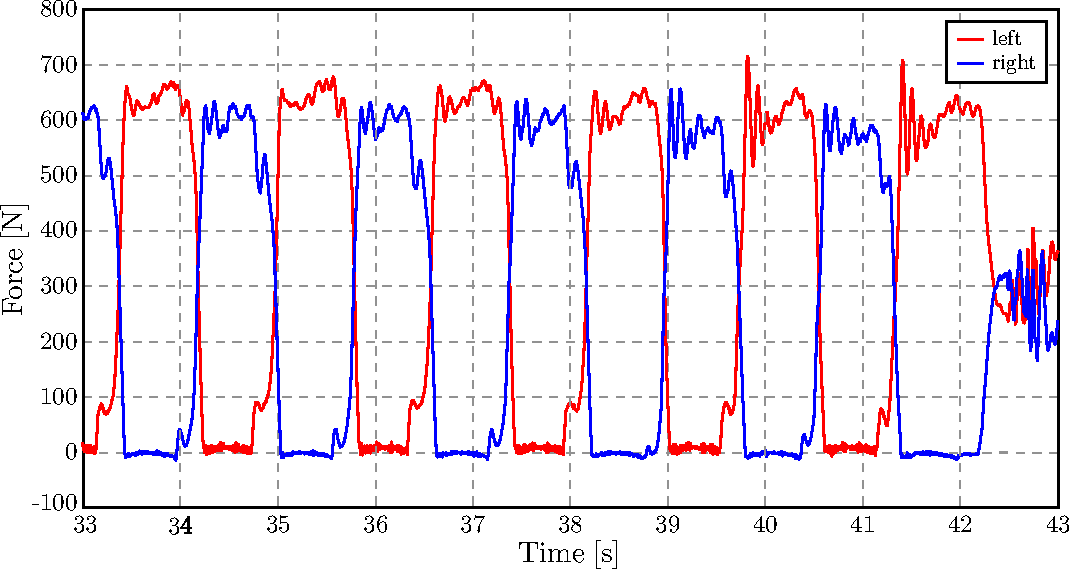
\includegraphics[trim={5.0cm 1.5cm 7.0cm 1.0cm}, clip, width=\textwidth , height=0.15\textheight]
      {hose_xp/force_Z_feet_withController_zoomEnd.pdf}
      %trim={<left> <lower> <right> <upper>}
      \end{center}
  \end{minipage}\\[-1ex]
%   
  \begin{minipage}{0.30\textwidth}
    \vspace*{2ex}
    \begin{itemize}
      \item Static Balance
      \item Feet flat
      \item (Self-)Collisions
    \end{itemize}
  \end{minipage}
%
{\color{txtcolor2}\vrule}
  \begin{minipage}{0.30\textwidth}
    \vspace*{2ex}
    \begin{itemize}
      \item PI controller :
    \end{itemize}
    \vspace*{-0.5cm}
    \begin{scriptsize}
    \begin{align*}
      \tikz[baseline]{
        \node[fill=txtcolor1,anchor=base] (v)
        { $ \mathbf{v}^{\mathrm{ref}} $ };
      }
      = &- \tikz[baseline]{
        \node[fill=txtcolor2,anchor=base] (l1)
        {$\lambda$};
      } \;
      \tikz[baseline]{
        \node[fill=txtcolor3,anchor=base] (e1)
        {$ \mathbf{e}_{ch} $};
      }
      %
      \\
      %    
      &- 
      \tikz[baseline]{
        \node[fill=txtcolor2,anchor=base] (l2)
        {$ \mathbf{\Lambda} $};  
      }
      \int \tikz[baseline]{
        \node[fill=txtcolor3,anchor=base] (e2)
        {$ \mathbf{e}_{ch} $};
      } dt
    \end{align*}
    \tikz[baseline]{
    \node[fill=txtcolor3,anchor=base] (e3)
      {$ \mathbf{e}_{ch} $};
    }
    $= 
    \begin{bmatrix}
      x_{ch} \\ y_{ch} \\ \theta_{ch}
    \end{bmatrix}
    -
    \begin{bmatrix}
      x^{des}_{ch} \\ y^{des}_{ch} \\ \theta^{des}_{ch}
    \end{bmatrix}
    $   
    \end{scriptsize}
  \end{minipage}
%
{\color{txtcolor2}\vrule}
  \begin{minipage}{0.30\textwidth}
    \vspace*{2ex}
    \begin{itemize}
    \item Hybrid Control
    \end{itemize}
    \vspace*{-0.5cm}
    \begin{scriptsize}
    \begin{align*}
      m & \tikz[baseline]{
        \node[fill=txtcolor1,anchor=base] (a)
        { $ \ddot{\bf lw}^{\alpha} $ };
      }
     + c \tikz[baseline]{
        \node[fill=txtcolor1,anchor=base] (v)
        {$ \dot{\bf lw}^{\alpha} $};
      } = 
      %
      \\
      %
      &\tikz[baseline]{
        \node[fill=txtcolor4,anchor=base] (flw)
        {$ {\bf f}_{lw}^{\alpha} $};
      } + 
      \tikz[baseline]{
        \node[fill=txtcolor2,anchor=base] (fd)
        {$ {\bf f}_{d}^{\alpha} $};
      } + 
      \tikz[baseline]{
        \node[fill=txtcolor3,anchor=base] (fpull)
        {$ {\bf f}_{pull}^{\alpha} $};
      }
      %
      \\
      %
      &\alpha \in \{x,z\}
      %
      \\
      %
      &\tikz[baseline]{
        \node[fill=txtcolor1,anchor=base] (a)
        { $ {\bf lw}^{y} $ };
      } = {\bf waist}^{y} + \text{offset}
    \end{align*}
    \end{scriptsize}
  \end{minipage}
%
\end{frame}

%%%%%%%%%%%%%%%%%%%%%%%%%%%%%%%%%%%%%%%%%%%%%%%%%%%%%%%%%%%%%%%%%%%%%%%%%%%%%%%%%%%%%%%

\begin{frame}{Full controller}
  \scalebox{0.7}{%!TEX root = ../../14-icra-RealTimeNMPC.tex

\tikzstyle{block} = [draw, fill=blue!20, rectangle,
    minimum height=2em, minimum width=5em, align=center]
\tikzstyle{sum} = [draw, fill=blue!20, circle, node distance=1cm]
\tikzstyle{input} = [coordinate]
\tikzstyle{output} = [coordinate]
\tikzstyle{pinstyle} = [pin edge={to-,thin,black}]

% The block diagram code is probably more verbose than necessary
\begin{tikzpicture}[auto, node distance=2cm,>=latex]

    % We start by placing the blocks
    \node [input]  at (0.0, 0.0) (input)  {};
    \node [input]  at (3, 0.0) (velocity) {};
    \node [input]  at (0.2, -2.8) (feedback)  {};
    \node [input]  at (16, -2.8) (feedback2)  {};
    \node []    at ( 0.0, 0.0) (sumin)  {};
    %\node [output]    at ( 15, 0.0) (sumout) {};
    \draw [fill=green,opacity=.2,text opacity=1] (3.5,1.5) rectangle (11.5,-2.7);
    \node at(10,-1.7) {\textcolor{green!20!black!100}{Stack of Task}};

    \node [block] at (4.6,-1.7) (lwc) {
        Left Wrist\\
        Hybrid\\
        Controller        
    };

    \node [block] at (1.7,0.0) (walking) {
        Walking \\
        Task    
    };

    \node [block] at (4.6,0) (wpg) {
        Walking\\
        Pattern\\
        Generator
    };
%    \node [block] at (4.2,0) (dyn) {
%        Dynamic\\
%        Filter
%    };
    \node [block] at (7.5,0) (ttt) {
        Task for\\
        Trajectory\\
        Tracking
    };
    
    \node [block] at (10.5,0) (qp) {
        HQP\\
        solver
    };

    \node [block] at (14.0, 0) (system) {
    		Robot Hardware\\
    		{\footnotesize Simulation/Robot}\\
    		and\\
    		{\footnotesize motion capture system}
    	};

    % PATHS
    	% Forward chaine
    \draw [draw,-] (input) -- node {\small ${\mathbf{p}}^{\,{\text {ref}}}$} (walking);
    
    \draw [draw,->] (walking) -- node {\small ${\mathbf v}^{\,{\text{ref}}}$} (wpg);
%    \draw [draw,- ] (walking) -- node {} (velocity);
    \draw [draw,->] (velocity) |- node {} (lwc);
%    \draw [->] (wpg) -- node {\small $c^{ref},f^{ref}$} (dyn);
%    \draw [->] (dyn) -- node {\small $\tilde{c}^{\,ref},f^{ref}$} (sot);
    \draw [->] (wpg) -- node [text width=0.8cm]{\small ${\mathbf{p}_c}^{\,{\text {ref}}}$ ${\mathbf{p}_f}^{\,{\text {ref}}}$} (ttt);
    \draw [->] (ttt) -- node [text width=0.8cm]{
    \small Tasks
    } (qp);
    \draw [->] (qp) -- node [text width=0.6cm]{\small ${\mathbf q}^{\,{\text{ref}}}$ $\dot{{\mathbf q}}^{\,{\text{ref}}}$} (system);
    
    \draw [->] (lwc) -| node [near start, above]{\small ${\mathbf{p}_{lw}}^{\,{\text {ref}}}$} (ttt);
    %\draw [->] (system) -- node {} (sumout);

    % Feedback chaine
%    \draw [- ] (dyn)      -| node {} (feedback);
%    \draw [->] (feedback) -| node {} (wpg);
    
    \draw [- ] (system.east)    -| node {} (feedback2);
    \draw [- ] (feedback2)  -- node [above]{\small $\mathbf{f}_{lw},\mathbf{p}_{w},\mathbf{p}_{lw},\mathbf{p}_{f}$} (feedback);
    \draw [->] (3.0,-2.8) |- node [near start, above]{} ([yshift=-0.2cm]lwc.west);
    \draw [->] (feedback) |- node [below=0.7cm, right]{\small $\mathbf{p}_{ch}$} ([yshift=-0.2cm]walking);

%    \draw [->] (dyn) -| node[above right] {\small $\hat{c}^{\,x,y,\theta}$, $\hat{f}^{\,\,x,y,\theta}$} (wpg);
\end{tikzpicture}
} \\
%

%  \textbf{\color{blue}Full feedback scheme}
%
\end{frame}

\begin{frame}{Complete motion}
  \begin{center}
    \movie[autostart,loop]{
    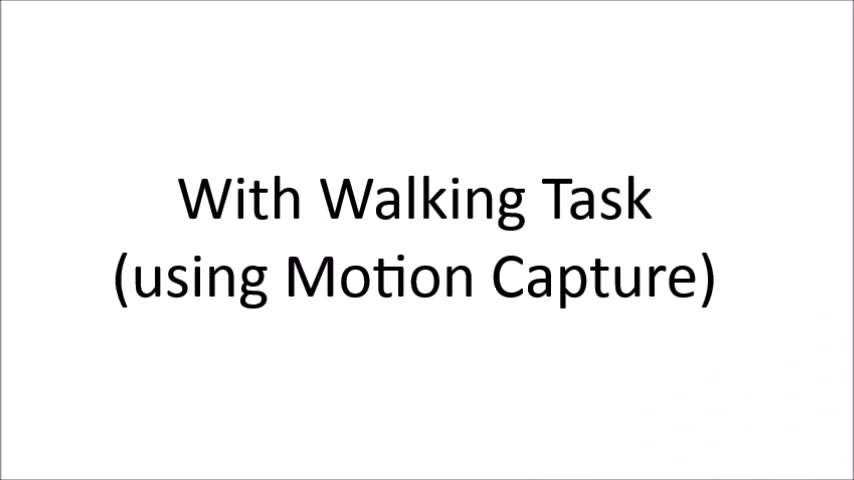
\includegraphics[width=0.9\linewidth, height=\textheight, keepaspectratio]
    {hose_xp/wholemotion.png}    
    }  
    {./videos/wholemotion.mpg}
  \end{center}
\end{frame}             % 5

\section{power-law}
\setcounter{subsection}{5}


\begin{frame}{Transferring the human power-law to humanoid robots}
  \vspace*{-0.5cm}
  \begin{itemize}
    \item Observation :
    \begin{itemize}
      \item Robots drift in curved trajectories
      \item Human moves according to the one-third power-law
    \end{itemize}
    \begin{center}
    \tikz[baseline]{\node[fill=txtcolor3,anchor=base]{$ v $};} =
    \tikz[baseline]{\node[fill=green!50,anchor=base]{$\left( \frac{1}{R} \right)$};}
    \textsuperscript{\tikz[baseline]{\node[fill=red!50,anchor=base]{$-\beta$};}}
    \end{center}
    \vspace*{-0.5cm}
    \scalebox{1}{\begin{tikzpicture}
    \node (zero) at (0,0) {};
    \filldraw [gray] ([xshift=-3cm,yshift=-2cm] zero) circle (2pt) + (6,0) circle (2pt);
    \node[color=gray] at ([xshift=-3.75cm,yshift=-2cm] zero) {Start};
    \node[color=gray] at ([xshift=3.75cm,yshift=-2cm] zero) {Goal};
    
    % Trajectory
    \draw[thick,color=red]
    (-3,-2) .. controls +(3,0) and +(-1,2) .. +(6,0);

      % Point in gray
      \filldraw [gray] ([xshift=1.75cm,yshift=-1.1262cm] zero) circle (2pt);
      % Name of the point: P
      \node at ([xshift=1.75cm,yshift=-0.75cm]zero) {$P$};


        % Osculting circle
        \draw[color=blue] (1.7,-2.125) circle (1cm);
        % Drawig Ray to the plot 
        \draw (1.7,-2.125) -- (1.75,-1.1262);
        % Ray label
        \node [fill=green!50] at (2.1,-1.8262) {$R$};
        % Tangent vector to the osculting circle along the trajectory (velocity vector)
        \draw (0.7512,-1.0762) -- (2.7488,-1.1762);

    % Speed
      \draw[-latex,thick,color=orange] (1.75,-1.1262) -- (2.4991,-1.1637)
      node[above] {$v$};

    \draw[-latex,thick,color=orange] (-3,-2) -- (-2.5,-2)
    node[above]{$v_{Start}$};
    
    \draw[-latex,thick,color=orange] (3.0,-2) -- (3.25,-2.5)
    node[below]{$v_{Goal}$};
\end{tikzpicture}}
    \item Does this one-third power law help humanoid robots to walk?
  \end{itemize}
\end{frame}

\begin{frame}{Drift compensation}
\vspace*{-0.8cm}  
  \begin{center}
    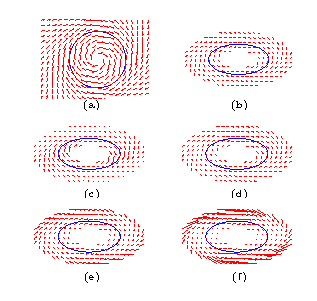
\includegraphics[height = 5.0cm]{two_third/morphing.pdf}
  \end{center}
  \vspace*{-0.5cm}
  \begin{itemize}
    \item Contracting vector field towards cyclic reference trajectories.
    \item (a) unit cycle oscillator, (b) elliptic morphing
    \item (c) $\rightarrow$ (f) $\beta=\{-\frac{1}{3},0,\frac{1}{3},\frac{2}{3}\}$
  \end{itemize}
\end{frame}

%\pgfdeclareimage[width=2.0cm]{VectorFields}{./images/Koroibot/EllipseBetaThird}
%\begin{frame}{Feedback controller}
%  \begin{center}
%      \begin{tikzpicture}%[show background grid]% every node/.style={draw,outer sep=0pt,thick}]
%
%    % Ellispe Reference
%    \node[rectangle,minimum width=2cm, minimum height=1cm,draw=blue!70,fill=blue!20] (ellipseref) at (4.0,3.25) {};
%    \node[ellipse,draw=blue,thick,minimum width=1cm,minimum height=0.5cm] at (4.0,3.25) {};
%    \node at (4.0,2.25) {Reference trajectory};
%
%    % Vector Field
%    \node[rectangle,minimum width=2cm, text width=2cm,minimum height=1cm,draw=blue!70,fill=blue!20,align=center] (vectorfields) at (0.0,0.0) 
%         {Vector Field\\
%           $\pgfuseimage{VectorFields}$};
%         %\node at (0.0,2.5) {$\gamma,\beta$};
%
%    % Walking Pattern Generator
%    \node[rectangle,minimum width=2cm, minimum height=1cm,draw=blue!70,fill=blue!20]  (wpg) at (5.4,1.0) {Walking Pattern Generator};
%
%    % Robot
%    \node[rectangle,minimum width=2cm, text width=3cm, align=center, minimum height=1cm,draw=blue!70,fill=blue!20] (sot) at (6.0,-1.0) 
%      {Stack-of-Tasks\\ Whole Body Motion Generator};
%
%    % Power Law
%    \node[rectangle,text width=2cm,align=center,minimum width=2cm, minimum height=1cm,draw=blue!70,fill=blue!20] (powerlaw) at (3.0,-1.0) {Power Law\\$\gamma,\beta$};
%    \path[->,>=stealth',draw=black] (vectorfields.314)-- node[below] {$\kappa$} (powerlaw.189);
%    \path[->,>=stealth',draw=black] (powerlaw.170)-- node[above] {$v$} (vectorfields.325);
%
%    % Robot
%    \node[rectangle,minimum width=2cm, minimum height=1cm,draw=blue!70,fill=blue!20] (robot) at (6.0,-3.0) {Robot};
%
%    % Localization
%    \node[rectangle,minimum width=2cm, minimum height=1cm,draw=blue!70,fill=blue!20] (localization) at (0.0,-3.0) {Localization};
%
%    %\path[->,>=stealth',draw=black] (0.0,2.25)-- (vectorfields.90);
%
%    % Links
%    \draw[->,>=stealth',draw=black] (ellipseref.180) -| (vectorfields.90);
%    \draw[->,>=stealth',draw=black] (vectorfields.42) -- node[above] {${\bf c}^*$} (wpg.180);
%    \path[->,>=stealth',draw=black] (wpg.320)-- node[left] {${\bf c}_{ref},{\bf z}_{ref},{\bf LF}_{ref},{\bf RF}_{ref}$}(sot);
%    \path[->,>=stealth',draw=black] (sot)-- node[right] {${\bf q}$} (robot);
%    \path[->,>=stealth',draw=black] (robot)-- node[below,font=\small] {Motion capture}(localization);
%    \path[->,>=stealth',draw=black] (localization)-- node[left] {${\bf w}$}(vectorfields);
%  \end{tikzpicture}
%  \end{center}
%\end{frame}

\begin{frame}{Results}
  \begin{center}
    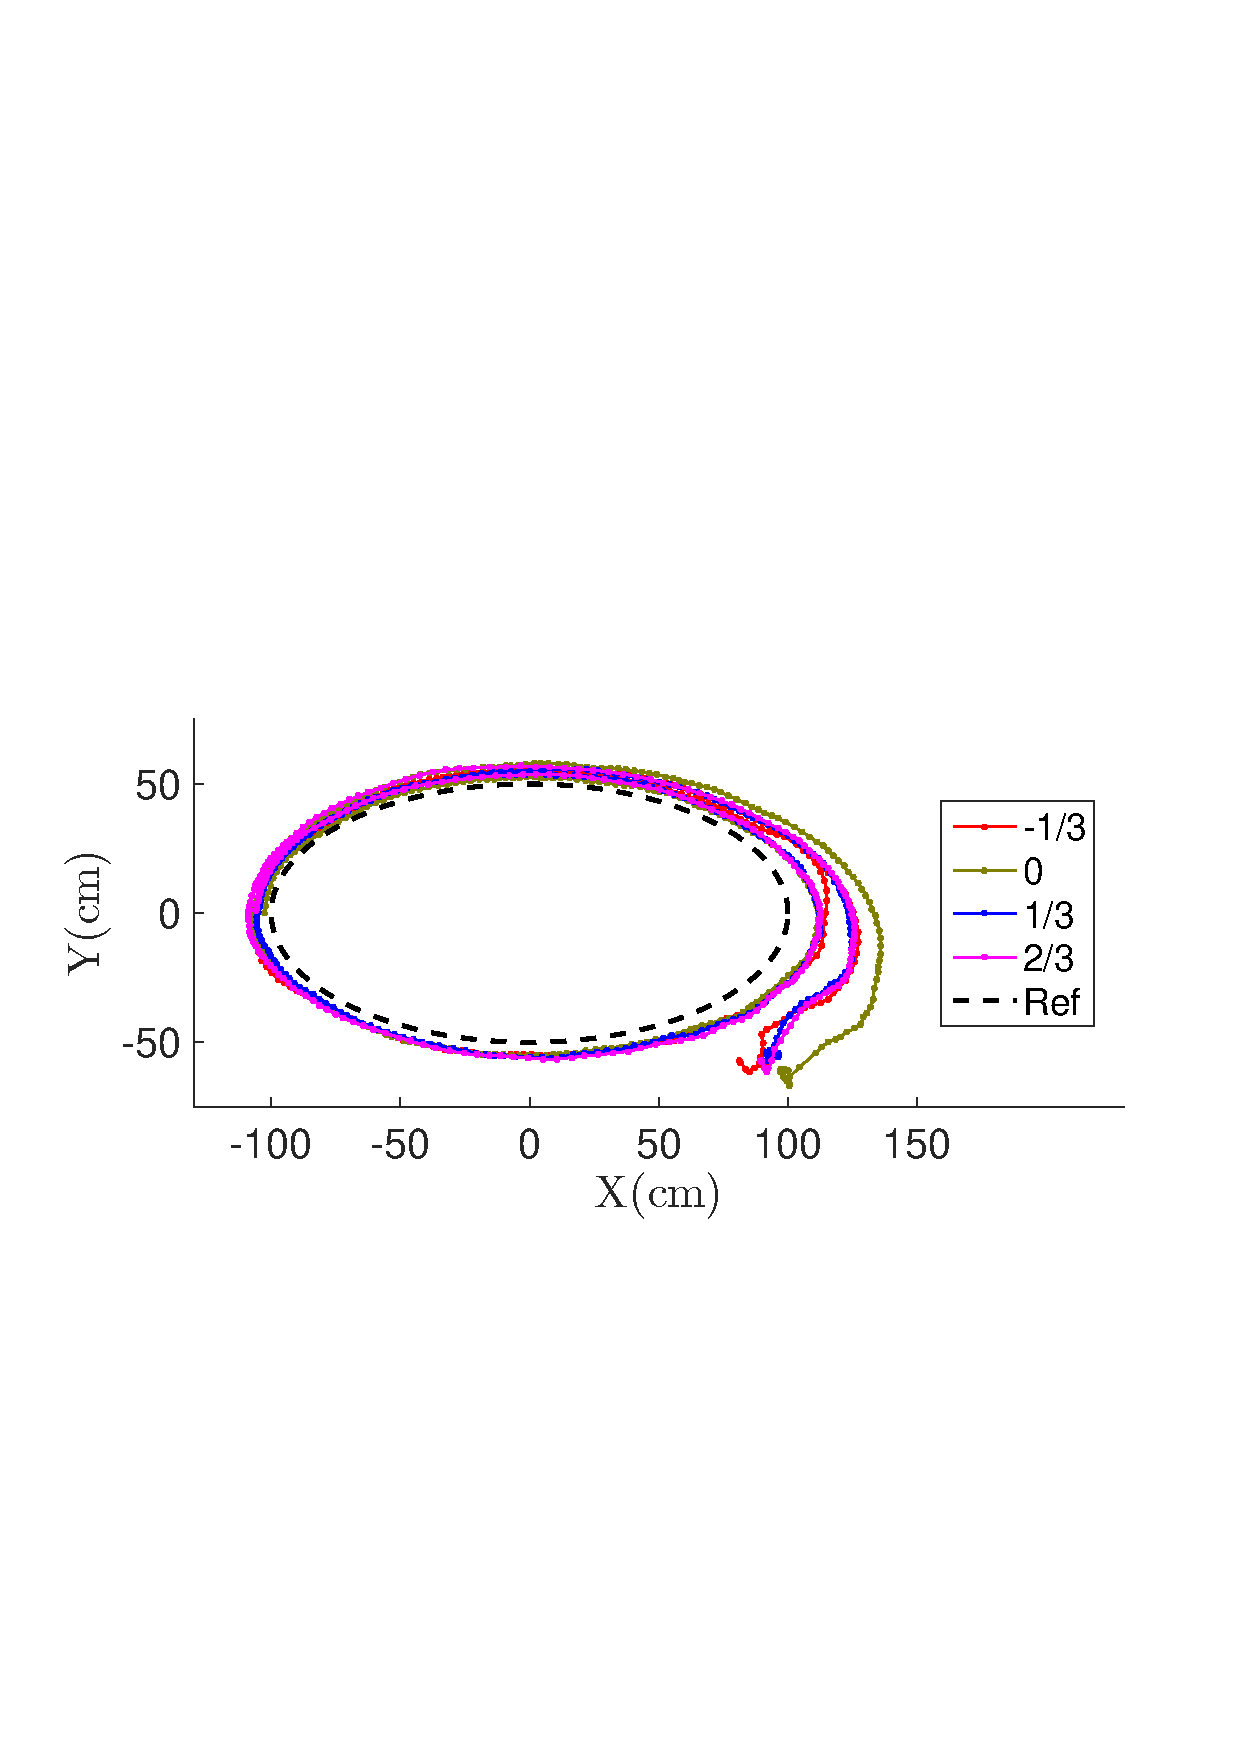
\includegraphics[trim={1.0cm 10.0cm 1.0cm 13.0cm}, clip,height = 3.0cm]
    {two_third/Fig5d_EXPshapesSymmetric.pdf}
    %trim={<left> <lower> <right> <upper>}
    \hfill
    \begin{table}[ht]
    	\centering 
	  \begin{tabular}{| c | c | c | c | c |c |} 
		  \hline 
		  Ref.~$\beta$        & $-\frac{1}{3}$  & $0$      & \textcolor{red}{$\frac{1}{3}$} & $\frac{2}{3}$   \\
		  \hline  
		  Norm     ($m$)        & $1.416$  & $0.950$  & \textcolor{red}{$0.642$} & $1.124$ \\   
		  Orientation ($deg$)   & $76.83$  & $89.60$  & \textcolor{red}{$60.45$} & $77.28$ \\ 
		  Tangential Force ($kN \; s$) & $21.93 $ & $23.54$  & \textcolor{red}{$19.80$} &$21.01$  \\ 
		  \hline 		  
	  \end{tabular}
  \end{table}
  \end{center}
  \blfootnote{(Karklinsky, \textbf{Naveau} et al. BioRob 2016)}
%  
%  Globally, the     values of the simulated motions reflect the ones of     the reference trajectory 
%
%The position of maximal speed on simulated trajectories is slightly shifted  (delayed)
%
%Unpredictably, for         ,  an oscillatory curvature-dependent speed profile is observed
%
%The controlled motions take more time than the reference movement. The higher     the faster the motion. 
\end{frame}





     % 5

\section{motion-primitives}
\setcounter{subsection}{6}

\begin{frame}{Learning Movement Primitives for the Humanoid Robot HRP2}
\framesubtitle{
  \textcolor{green!30!black!80}
  {
    (A. Mukovskiy, JRAS 2016)
  }
}
  %\vspace*{-0.8cm}  
  \begin{center}
    \scalebox{0.7}{\newcommand{\picturefontsize}{\LARGE}
\newcommand{\pictureLineWidth}{0.8mm}

% For every picture that defines or uses external nodes, you'll have to
% apply the 'remember picture' style. To avoid some typing, we'll apply
% the style to all pictures.
\tikzstyle{every picture}+=[remember picture]
\tikzstyle{na} = [baseline=-.5ex]

\def\localarrow{
\begin{tikzpicture}
\path[draw=blue!50,fill=blue!40] (0,0.125) -- (1.0,0.125) -- (1.0,0.25) -- (1.25,0.0) -- (1.0,-0.25) -- (1.0,-0.125) -- (0.0,-0.125) -- (0.0,0.125);
\end{tikzpicture}
}

\begin{tikzpicture}%[show background grid]% every node/.style={draw,outer sep=0pt,thick}]

% Rectangle
\node (trainingdata) [text centered, shape=rectangle,rounded corners,draw=blue!50,fill=blue!10,thick,text width=2cm, minimum height=3cm]
  at (0.0,-0.5) {\textbf{Training data} extracted from human motion};

\node (movementprimitives) [text centered, shape=rectangle,rounded corners,draw=blue!50,fill=blue!10,thick,text width=2cm, minimum height=3cm]
  at (4.0,-0.5) {\textbf{Movement primitives} segmentation and retargeting};

\node (movementsynthesis) [text centered, shape=rectangle,rounded corners,draw=blue!50,fill=blue!10,thick,text width=2cm, minimum height=3cm]
  at (8.0,-0.5) {\textbf{Movement synthesis} using oscillators};

\node (robotcontrol) [text centered, shape=rectangle,rounded corners,draw=blue!50,fill=blue!10,thick,text width=2cm, minimum height=3cm]
  at (12.0,-0.5) {\textbf{Robot control}\\Walking Pattern Generator,\\ Stack of Tasks,\\ Robot};

\node (firstarrow) at (2.0,0.25) {\localarrow };

\node (sndarrow) at (6.0,0.25) {\localarrow };

\node (thrdarrow) at (10.,0.25) {\localarrow };

\node[rotate=180] (rfirstarrow) at (2.0,-1.25) {\localarrow };
\node[rotate=180] (rsndarrow) at (6.0,-1.25) {\localarrow };
\node[rotate=180] (rthrdarrow) at (10.,-1.25) {\localarrow };

\node (offline1) at ( 2.0,-0.5) {Off line};
\node (offline2) at ( 6.0,-0.5) {Off line};
\node (offline1) at (10.0,-0.5) {On line};

\end{tikzpicture}
}
  \end{center}
%  
\end{frame}

\begin{frame}{Implementation on HRP-2}
  %\vspace*{-0.8cm}  
  \begin{center}
    \scalebox{0.7}{%!TEX root = ../../14-icra-RealTimeNMPC.tex

\tikzstyle{block} = [draw=blue!50, fill=blue!20, rectangle,
    minimum height=2em, minimum width=5em, align=center]
\tikzstyle{point} = [coordinate]
\tikzstyle{pinstyle} = [pin edge={to-,thin,black}]

\definecolor{KPS}{RGB}{204 ,  85 , 0}% corail
\definecolor{SBG}{RGB}{222, 152, 22 }% melon
\definecolor{WPG}{RGB}{231 ,  62 , 1}% orange 
\definecolor{SOT}{RGB}{179, 103, 0}% cuivre
\definecolor{ROB}{RGB}{173, 79, 9} % roux
\definecolor{EST}{RGB}{255, 127, 0}

% The block diagram code is probably more verbose than necessary
\begin{tikzpicture}[auto, scale=1.0]
  \draw [fill=green,opacity=.1,text opacity=1] (2.2,1.0) rectangle (14,-2.2);
  \node at(11,-2.0) {\textcolor{green!20!black!100}{Stack of Task}};

    \node [block, text depth=0.7cm, minimum width=2.0cm] at (10.0,-3.0) (robot) {
        Robot
    };
    \node [block, text opacity=1, opacity=0, font=\small, minimum width=1.1cm ] at ([yshift=-0.2cm]robot.center){
      (position \\
      control)
    };
%%%%
    \node [block,  text depth=0.8cm, minimum width=3.0cm] at (5.0,-3.0) (estimator) {
      Estimator 
    };
    \node [block, text opacity=1, opacity=0, draw=white, font=\small, minimum width=1cm ] at ([yshift=-0.2cm]estimator.center){
      (robot and objects\\
      relative positions)
    };
%%%%
    \node [block,  minimum width=0.1cm] at (3.5,-1.0) (wpg) {
        Walking\\
        Pattern\\
        Generator
    };
%%%%
    \node [block,  minimum width=0.1cm, text depth = 0.18cm] at (7.0,-1.0) (dyn) {
        \\[0.1cm]
        Dynamic\\
        Filter
    };
%%%%%
    \node [block,  text depth = 0.7cm, minimum width=2.0cm] at (10.5,-0.5) (sot) {
      \\[0.1cm]
      Task for\\
      Trajectory\\
      Tracking
    };
%%    \node [block, text opacity=1, opacity=0, draw=white, font=\footnotesize, minimum width=1.5cm ] at ([yshift=-0.3cm]sot.center){
%%      (generalized\\
%%      inverse\\
%%      kinematics,\\
%%      SoT)
%    };
    \node [block,  text depth = 1.0cm, minimum width=1.0cm] at (13.1,-0.5) (qp){
      \\[0.5cm]      
      QP\\solver
    };
%%%%  
    \node [block,  minimum width=0.1cm] at (0.0, 0.0) (kps) {
    		Kinematic \\
      Pattern \\
      Synthesis
    	};
%%%%%%%%%%%%%%%%%%%%%%%%%%%%%%%%%%%%%%%%%%%%%%%%%%%%%%%%%%%%%%%%%%%%%%%%%%%%%%%%%%%%%%%%%%
    % PATHS
    	% Forward chaine
    	\node [point] at ([xshift=-0.5cm]wpg.west) (walkingwest) {};
    \draw [ - ] ([yshift=-0.3cm]kps) -| node {} (walkingwest);
    \draw [ ->] (walkingwest) |- node [left] {\small $[{\mathbf v}^{\,{\text{ref}}}\;,\;{\mathbf \omega}^{\,{\text{ref}}}]$} (wpg.west);
%%%%    
    	\node [point] at ( $(dyn.west) + (-0.4,1.0)$ ) (dynwest) {};
    \draw [ - ] ([yshift=+0.1cm]kps) -- node  [above] {\small ${\mathbf q}^{\,{\text{upper body}}}$} (dynwest);
    \draw [ ->] (dynwest) |- node {} ([yshift=+0.3cm]dyn.west);    
    \draw [ ->] (dynwest) |- node {} ([yshift=+0.5cm]sot.west);
%%%%
    \draw [->] ([yshift=-0.1cm]wpg.east) -- node [below , font=\small] {} ([yshift=-0.1cm]dyn.west);
    \node [block, text opacity=1, opacity=0, font=\scriptsize, minimum width=0.01cm] at ($(dyn.west) + (-0.9,-0.7)$){
      CoM$^{ref,{\bf 1}}$ \\ ZMP$^{ref}$ \\ Feet$^{ref}$
    };
%%%%
    \draw [->] (dyn.east) -- node {} ([yshift=-0.5cm]sot.west);
    \node [block, text opacity=1, opacity=0, font=\scriptsize, minimum width=0.01cm] at ($(sot.west) + (-0.9,-1.1)$){
      CoM$^{ref,{\bf 2}}$ \\ ZMP$^{ref}$ \\ Feet$^{ref}$
    };
    
    \draw [draw,->] (sot) -- node {\small Tasks} (qp.west);

   	% Feedback chaine
    	\node [point] at ($(sot.east) + (0.1,0.0)$) (soteast) {};
    \draw [draw,->] (qp) |- node {\small ${\mathbf q},\dot{{\mathbf q}},\ddot{{\mathbf q}}$} (robot);
    
    \draw [draw,->] (robot) -- node {\small sensors data} (estimator);
    
    \draw [draw,->] (estimator) -| node [below right = 0.0cm and 0.5cm]{\small scene parameters} ($(kps.south)+ (-0.1,0.0)$);

    
%%%%%%%%%%%%%%%%%%%%%%%%%%%%%%%%%%%%%%%%%%%%%%%%%%%%%%%%%%%%%%%%%%%%%%%%%%%%%%%%%%%%%%%%5
\end{tikzpicture}

}
  \end{center}
%  
  \begin{itemize}
    \item The upper body is learned from humans.
    \item The lower body is computed via NMPC.
    \item The Dynamic Filter links them.
  \end{itemize}
\end{frame}

\begin{frame}{Effect of the dynamic filter}
\vspace*{-0.6cm}
  \begin{center}
    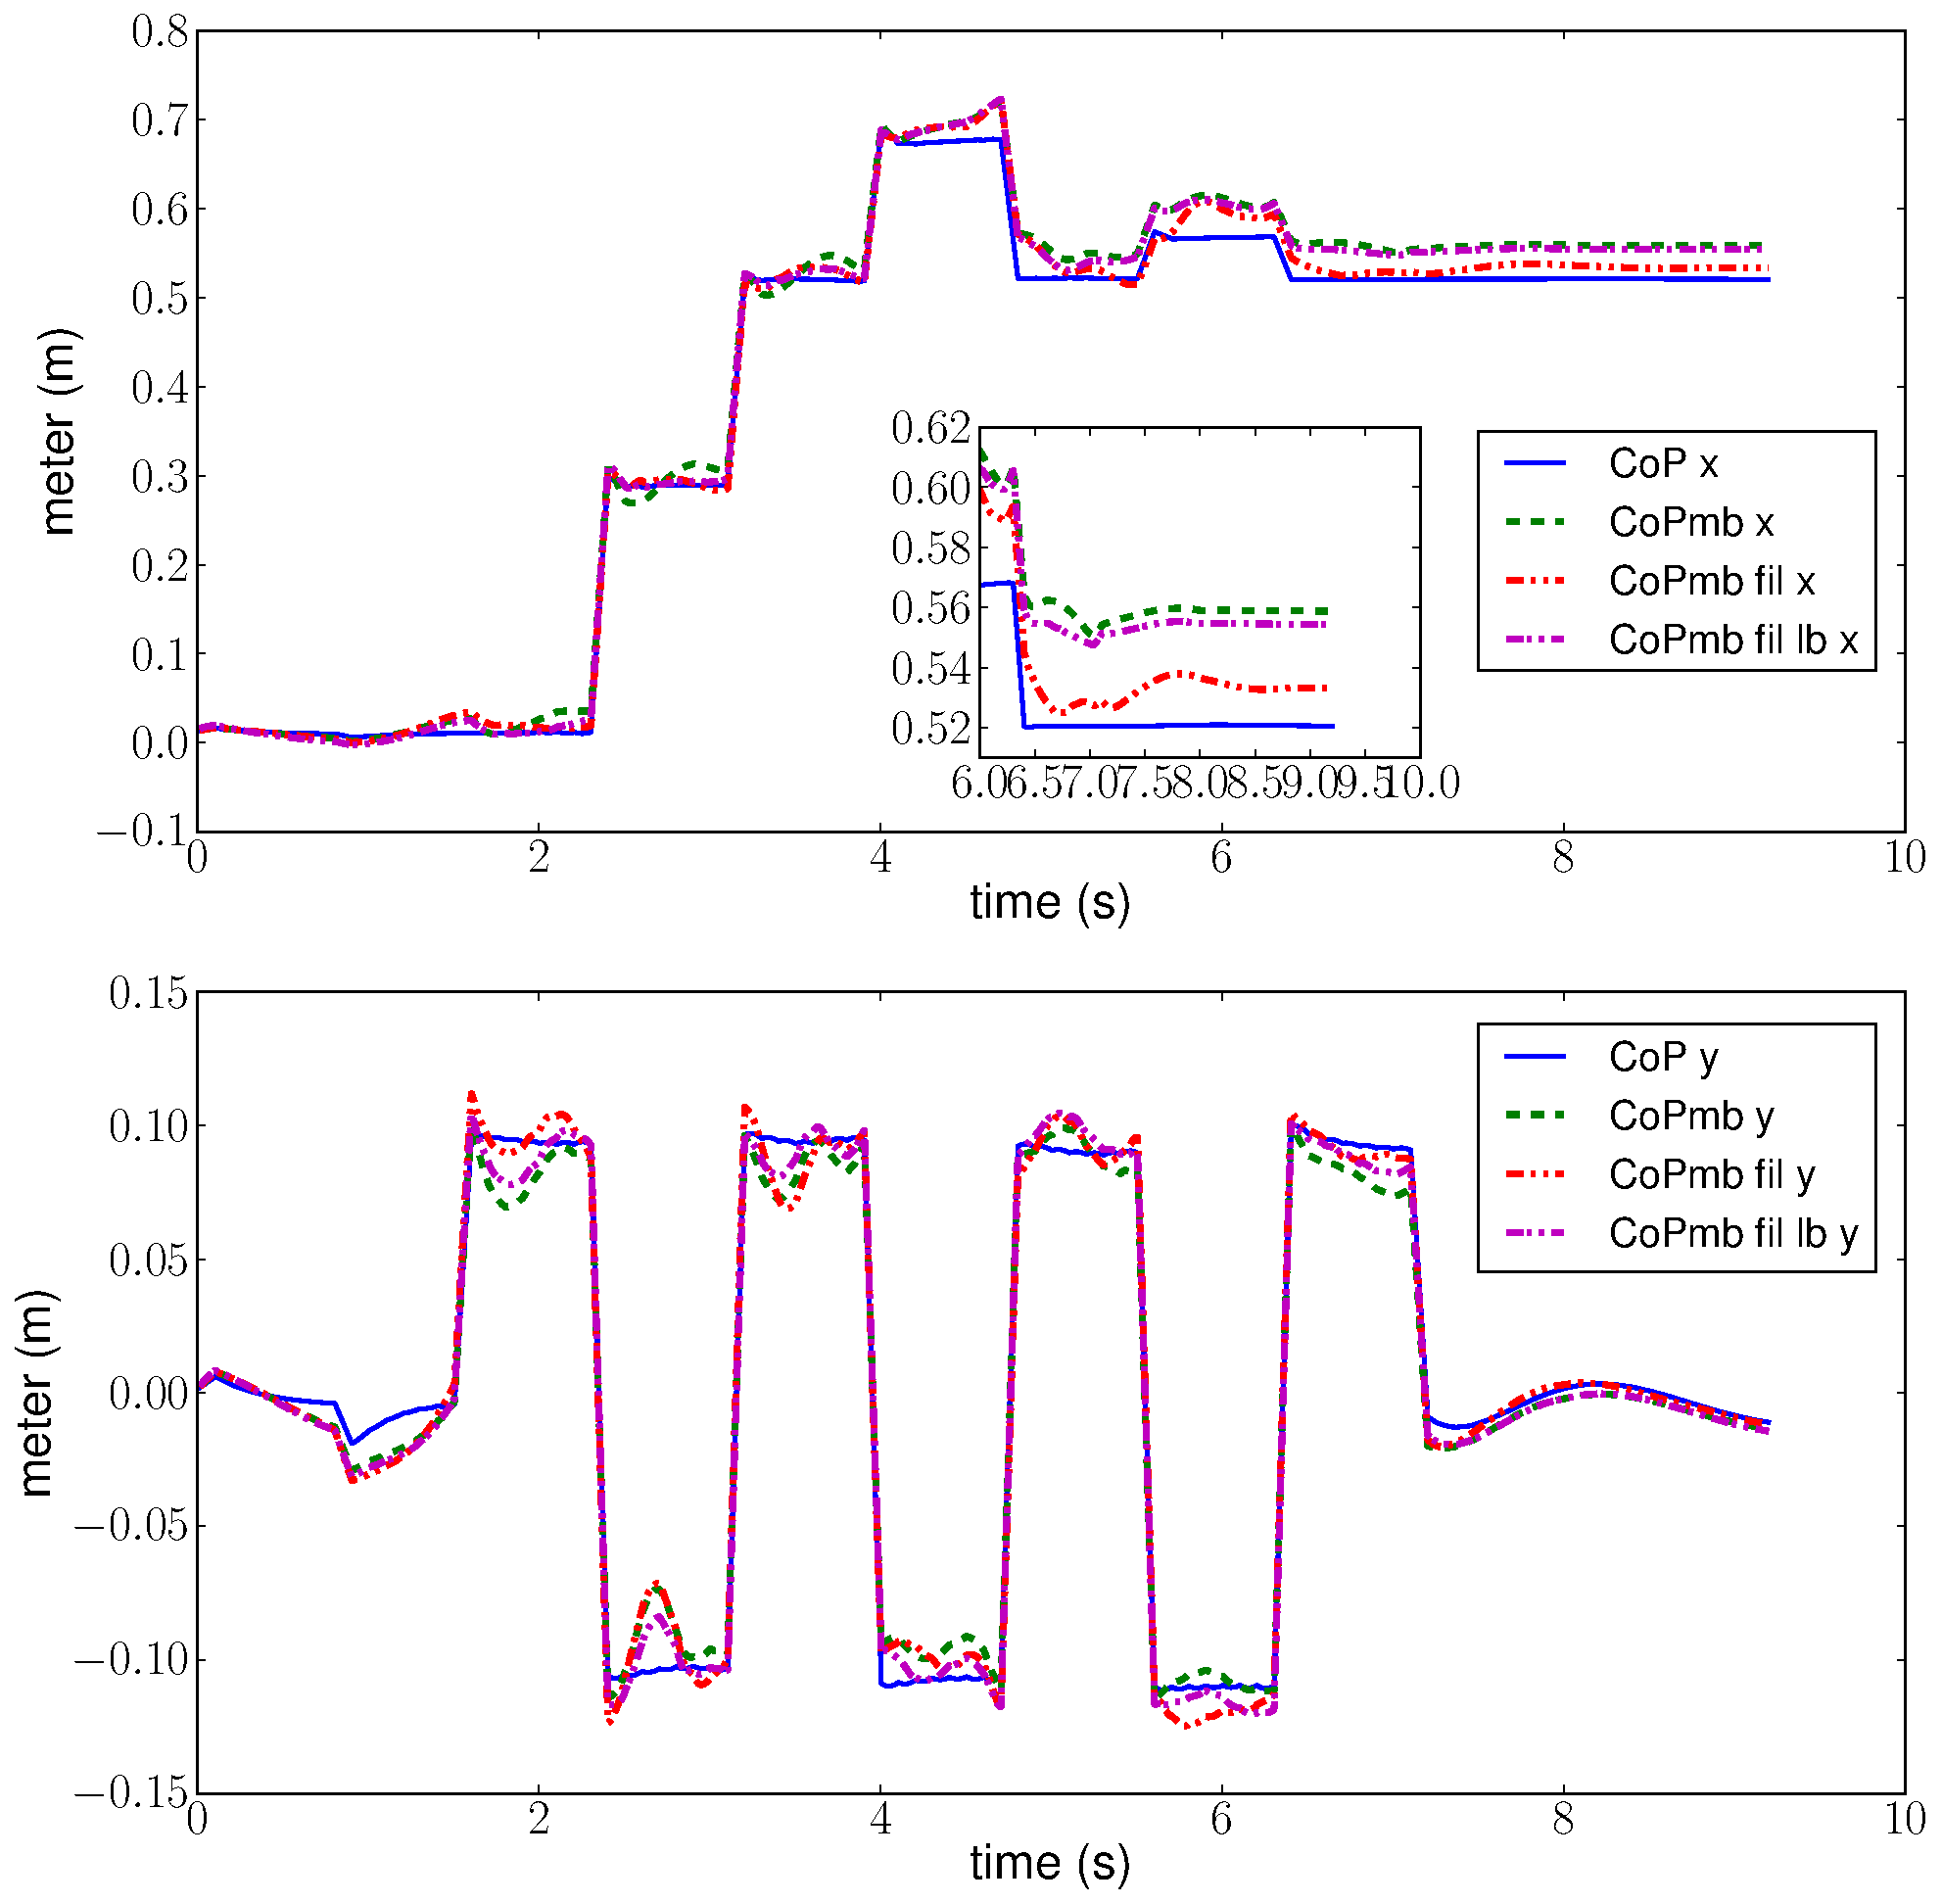
\includegraphics[height=0.9\textheight, keepaspectratio]
      {motion_primitives/copmb.pdf}    
  \end{center}
\end{frame}


\begin{frame}{Motion on HRP-2}
  \begin{center}
    \movie[autostart,loop]{
    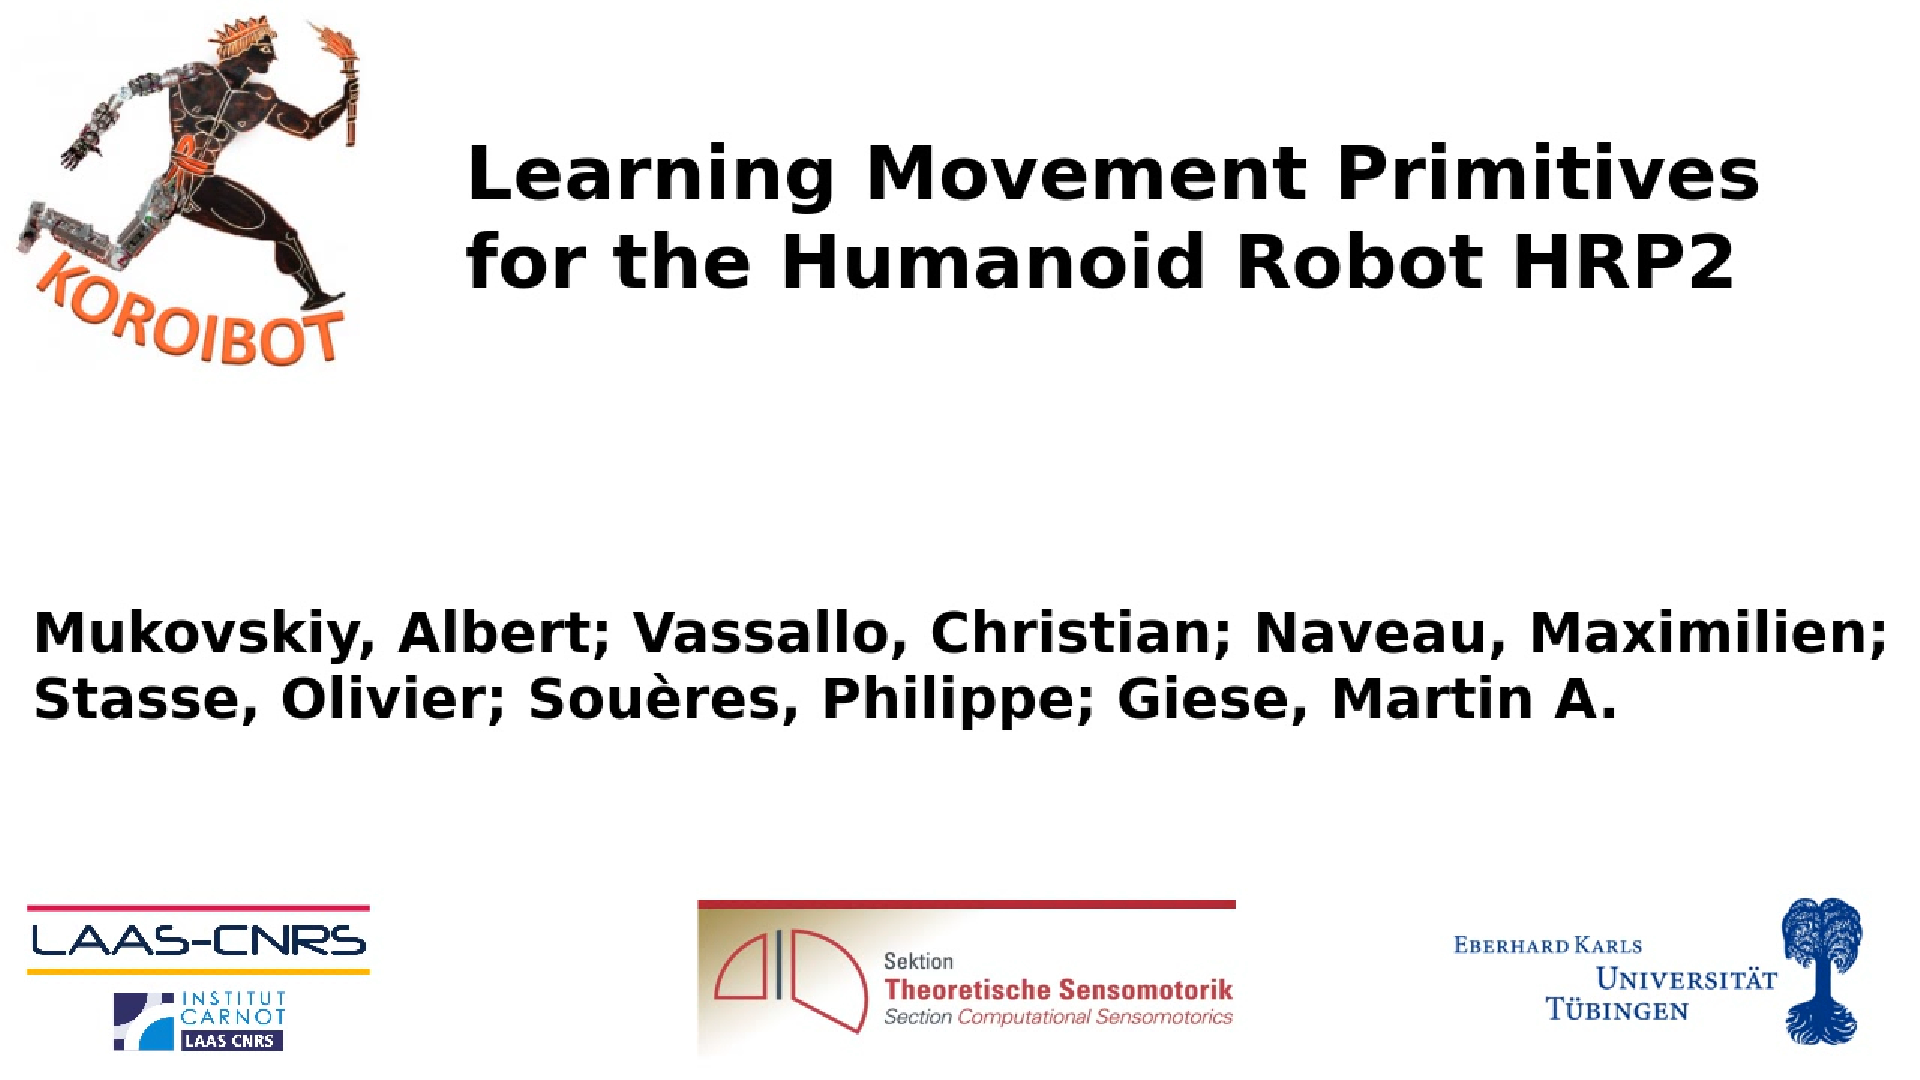
\includegraphics[width=0.9\linewidth, keepaspectratio]
      {motion_primitives/16-mukovskiy-elsarticle.png}    
    }  
    {./videos/16-mukovskiy-elsarticle.mp4}
  \end{center}
\end{frame}


       % 5

\section{airbus-application}
\setcounter{subsection}{7}

\begin{frame}{HRP-2 as Universal Worker\\Proof of Concept}
\framesubtitle{
  \textcolor{green!30!black!80}
  {
    (O. Stasse, Humanoids 2014)
  }
}
  \begin{center}
    \movie[autostart,loop]{
    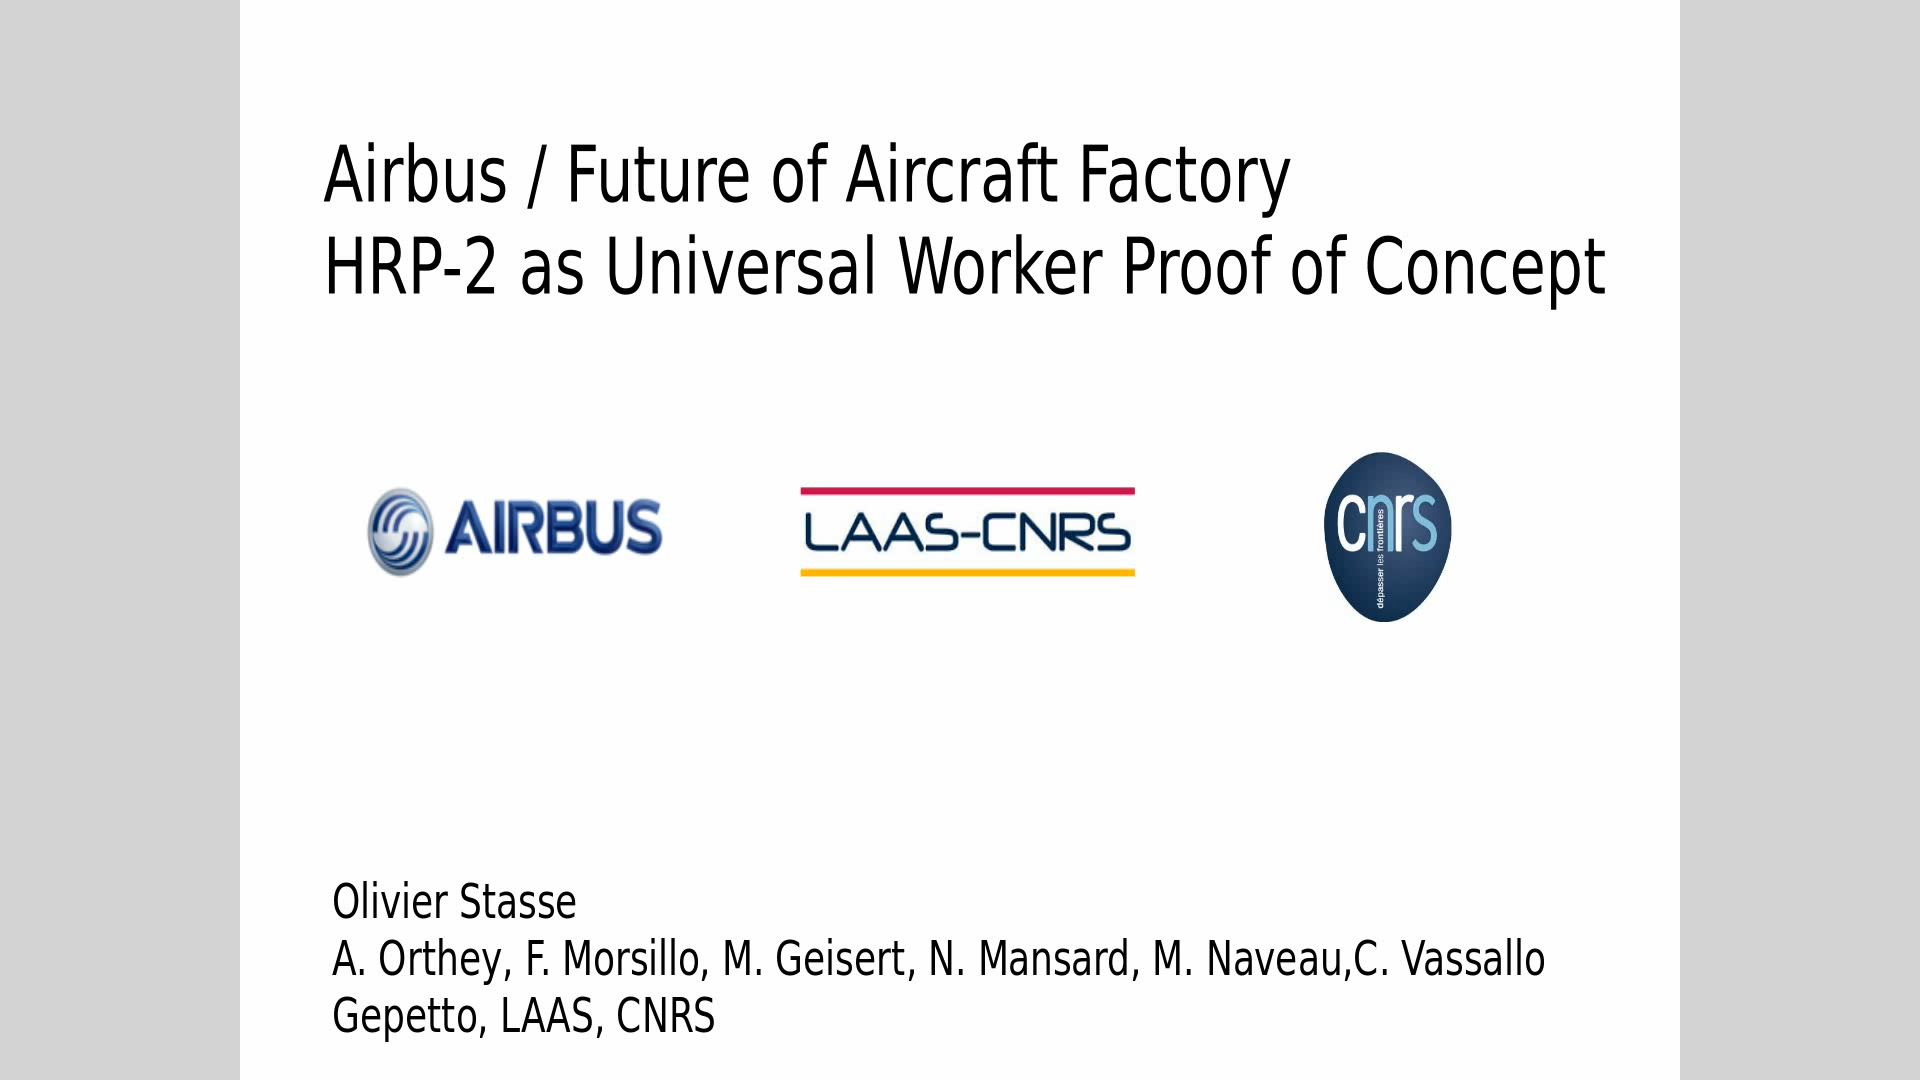
\includegraphics[width=0.85\linewidth, keepaspectratio]
      {poc_airbus/PocAirbus2013_12_Short.png}    
    }  
    {./videos/PocAirbus2013_12_Short.wmv}
  \end{center}
\end{frame}


            % 5

\section{conclusion}
\setcounter{subsection}{8}

\begin{frame}{Conclusion}
\framesubtitle{Main contributions :}
\begin{itemize}
  \item Implementation of the dynamic filter
  \begin{itemize}
    \item Fusion of human extracted motion primitives and optimal control for whole body   motion generation.
  \end{itemize}
  \item Novel reactive nonlinear walking pattern generator run in 1$ms$ on HRP-2
  \begin{itemize}
    \item Application of the walking pattern generator for pulling a hose.
    \item Introduction of the one-third power law in the humanoid robot locomotion.
  \end{itemize}
  \item Two multicontact pattern generator using the centroidal dynamics
\end{itemize}
\end{frame}

\begin{frame}{Conclusion}
\framesubtitle{Perspectives :}
\begin{itemize}
  \item Pursue the  work on generalized locomotion by determining 3D trajectories for end effectors and proper kinematic constraints.
  
  [Herdt 2010]
  \vspace*{1cm}
  \item Increase the versatility of the walking by using mixed-integer optimization. [Deits 2014]
\end{itemize}
\end{frame}
               % 5

\begin{frame}{The End}
\vspace*{-0.5cm}
\begin{center}
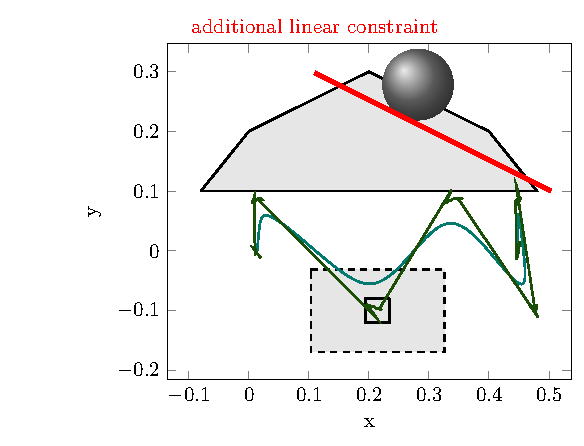
\includegraphics[width=0.4\textwidth, height=0.25\textheight, keepaspectratio]
  {./images/tikz/convexHullsplusObstacles2}
\hspace*{1cm}
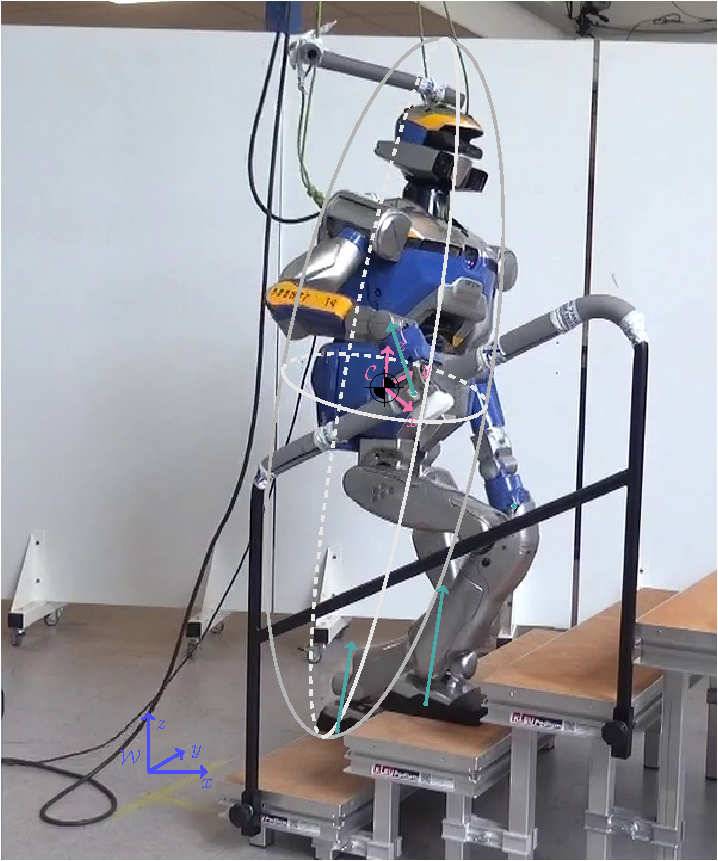
\includegraphics[width=0.4\textwidth, height=0.25\textheight, keepaspectratio]
  {multicontact/cover.pdf}\\
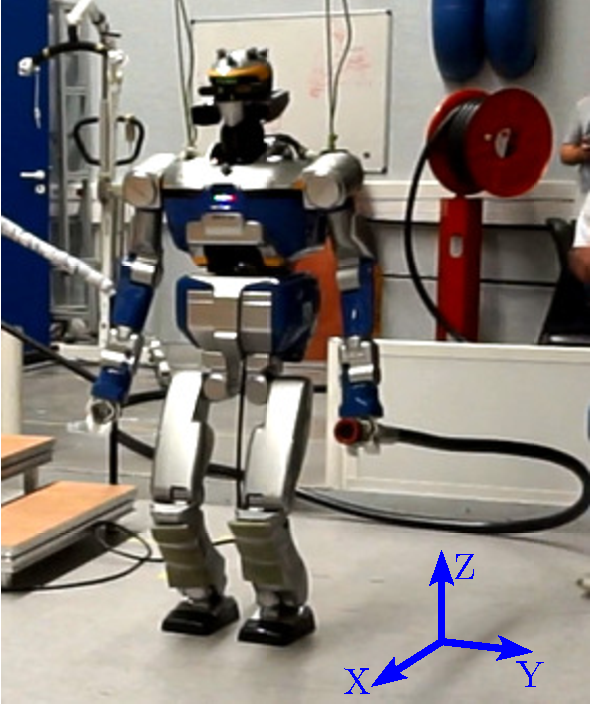
\includegraphics[width=0.4\textwidth, height=0.25\textheight, keepaspectratio]
  {hose_xp/coordinates.pdf}
\scalebox{0.7}{\begin{tikzpicture}
    \node (zero) at (0,0) {};
    \filldraw [gray] ([xshift=-3cm,yshift=-2cm] zero) circle (2pt) + (6,0) circle (2pt);
    \node[color=gray] at ([xshift=-3.75cm,yshift=-2cm] zero) {Start};
    \node[color=gray] at ([xshift=3.75cm,yshift=-2cm] zero) {Goal};
    
    % Trajectory
    \draw[thick,color=red]
    (-3,-2) .. controls +(3,0) and +(-1,2) .. +(6,0);

      % Point in gray
      \filldraw [gray] ([xshift=1.75cm,yshift=-1.1262cm] zero) circle (2pt);
      % Name of the point: P
      \node at ([xshift=1.75cm,yshift=-0.75cm]zero) {$P$};


        % Osculting circle
        \draw[color=blue] (1.7,-2.125) circle (1cm);
        % Drawig Ray to the plot 
        \draw (1.7,-2.125) -- (1.75,-1.1262);
        % Ray label
        \node [fill=green!50] at (2.1,-1.8262) {$R$};
        % Tangent vector to the osculting circle along the trajectory (velocity vector)
        \draw (0.7512,-1.0762) -- (2.7488,-1.1762);

    % Speed
      \draw[-latex,thick,color=orange] (1.75,-1.1262) -- (2.4991,-1.1637)
      node[above] {$v$};

    \draw[-latex,thick,color=orange] (-3,-2) -- (-2.5,-2)
    node[above]{$v_{Start}$};
    
    \draw[-latex,thick,color=orange] (3.0,-2) -- (3.25,-2.5)
    node[below]{$v_{Goal}$};
\end{tikzpicture}}\\
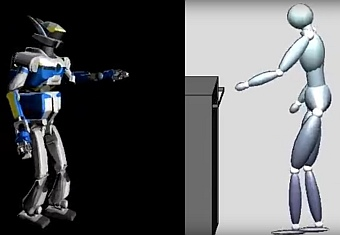
\includegraphics[width=0.4\textwidth, height=0.25\textheight, keepaspectratio]
  {motion_primitives/RobotAvatarjpg2.jpg}
\hspace*{1cm}
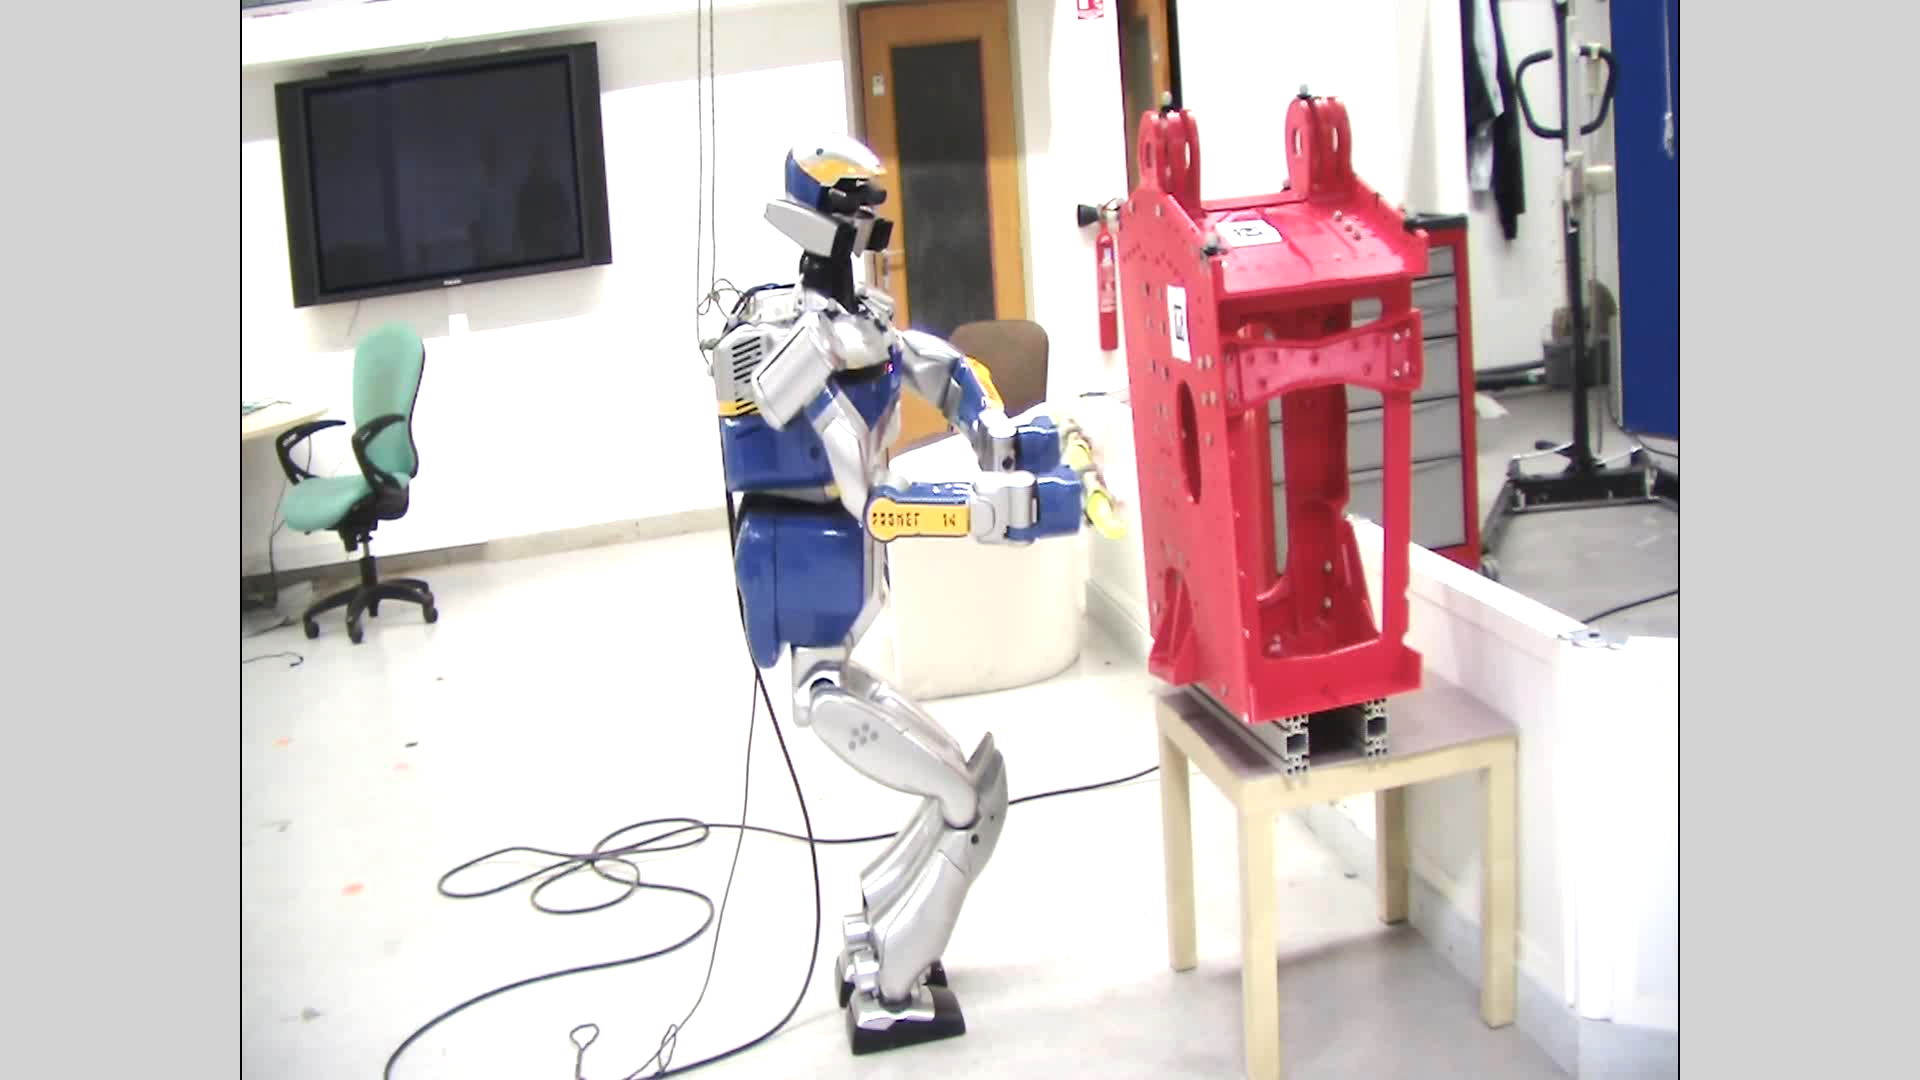
\includegraphics[width=0.4\textwidth, height=0.25\textheight, keepaspectratio]
{poc_airbus/PocAirbusCapture.png}
\end{center}
\end{frame}

\end{document}